%
% FH Technikum Wien
% !TEX encoding = UTF-8 Unicode
%
% Erstellung von Master- und Bachelorarbeiten an der FH Technikum Wien mit Hilfe von LaTeX und der Klasse TWBOOK
%
% Um ein eigenes Dokument zu erstellen, müssen Sie folgendes ergänzen:
% 1) Mit \documentclass[..] einstellen: Master- oder Bachelorarbeit, Studiengang und Sprache
% 2) Mit \newcommand{\FHTWCitationType}.. Zitierstandard festlegen (wird in der Regel vom Studiengang vorgegeben - bitte erfragen)
% 3) Deckblatt, Kurzfassung, etc. ausfüllen
% 4) und die Arbeit schreiben (die verwendeten Literaturquellen in Literatur.bib eintragen)
%
% Getestet mit TeXstudio mit Zeichenkodierung ISO-8859-1 (=ansinew/latin1) und MikTex unter Windows
% Zu beachten ist, dass die Kodierung der Datei mit der Kodierung des paketes inputenc zusammen passt!
% Die Kodierung der Datei twbook.cls MUSS ANSI betragen!
% Bei der Verwendung von UTF8 muss dnicht nur die Kodierung des Dokuments auf UTF8 gestellt sein, sondern auch die des BibTex-Files!
%
% Bugreports und Feedback bitte per E-Mail an latex@technikum-wien.at
%
% Versionen
% *) V0.7: 9.1.2015, RO: Modeline angepasst und verschoben
% *) V0.6: 10.10.2014, RO: Weitere Anpassung an die UK
% *) V0.5: 8.8.2014, WK: Literaturquellen überarbeitet und angepasst
% *) V0.4: 4.8.2014, WK: Initalversion in SVN eingespielt
%
\documentclass[BIF,Bachelor,nenglish]{twbook}%\documentclass[Bachelor,BMR,ngerman]{twbook}
\usepackage[utf8]{inputenc}
\usepackage[T1]{fontenc}
\usepackage{float}
\usepackage{pgfplots}
%
% Bitte in der folgenden Zeile den Zitierstandard festlegen
\newcommand{\FHTWCitationType}{IEEE} % IEEE oder HARVARD möglich - wenn Sie zwischen IEEE und HARVARD wechseln, bitte die temorären Dateien (aux, bbl, ...) löschen
%
\ifthenelse{\equal{\FHTWCitationType}{HARVARD}}{\usepackage{harvard}}{\usepackage{bibgerm}}

%
% Bei Bedarf bitte hier die Syntax-Highlightings anpassen
%
\usepackage[final]{listings}
\lstset{captionpos=b, numberbychapter=false,caption=\lstname,frame=single, numbers=left, stepnumber=1, numbersep=2pt, xleftmargin=15pt, framexleftmargin=15pt, numberstyle=\tiny, tabsize=3, columns=fixed, basicstyle={\fontfamily{pcr}\selectfont\footnotesize}, keywordstyle=\bfseries, commentstyle={\color[gray]{0.33}\itshape}, stringstyle=\color[gray]{0.25}, breaklines, breakatwhitespace, breakautoindent}
\lstloadlanguages{[ANSI]C, C++, [gnu]make, gnuplot, Matlab}

%Formatieren des Quellcodeverzeichnisses
\makeatletter
% Setzen der Bezeichnungen für das Quellcodeverzeichnis/Abkürzungsverzeichnis in Abhängigkeit von der eingestellten Sprache
\providecommand\listacroname{}
\@ifclasswith{twbook}{english}
{%
    \renewcommand\lstlistingname{Code}
    \renewcommand\lstlistlistingname{List of Code}
    \renewcommand\listacroname{List of Abbreviations}
}{%
    \renewcommand\lstlistingname{Quellcode}
    \renewcommand\lstlistlistingname{Quellcodeverzeichnis}
    \renewcommand\listacroname{Abkürzungsverzeichnis}
}
% Wenn die Option listof=entryprefix gewählt wurde, Definition des Entyprefixes für das Quellcodeverzeichnis. Definition des Macros listoflolentryname analog zu listoflofentryname und listoflotentryname der KOMA-Klasse
\@ifclasswith{scrbook}{listof=entryprefix}
{%
    \newcommand\listoflolentryname\lstlistingname
}{%
}
\makeatother
\newcommand{\listofcode}{\phantomsection\lstlistoflistings}

% Die nachfolgenden Pakete stellen sonst nicht benötigte Features zur Verfügung
\usepackage{blindtext}

%
% Einträge für Deckblatt, Kurzfassung, etc.
%
\title{Comparison between Microservice and Monolithic Web \ac{API} in a Cloud Environment}
\author{Florian Feka}
\studentnumber{1910257104}
%\author{Titel Vorname Name, Titel\and{}Titel Vorname Name, Titel}
%\studentnumber{XXXXXXXXXXXXXXX\and{}XXXXXXXXXXXXXXX}
\supervisor{Marvin Kosmider, MSc.}
%\supervisor[Begutachter]{Titel Vorname Name, Titel}
%\supervisor[Begutachterin]{Titel Vorname Name, Titel}
%\secondsupervisor{Titel Vorname Name, Titel}
%\secondsupervisor[Begutachter]{Titel Vorname Name, Titel}
%\secondsupervisor[Begutachterinnen]{Titel Vorname Name, Titel}
\place{Vienna}
\kurzfassung{Neben der monolithischen Architektur welche für lange Zeit die primäre Art war Software zu schreiben insbesondere in der Webentwicklung, haben weitere Architekturen hervor gestochen die sich mit der Zeit immer verbreiten. Gleichzeitig wird das Thema Cloud und die vielen Services die diese bietet immer mehr Thema und damit auch die Frage welche Architektur man verwenden soll, wenn man in die Cloud will. Die Frage besteht welche der zwei Architekturen nun in der Cloud performanter ist und besser skaliert. Es wurden schon Arbeiten veröffentlicht in denen die Monolithische Architektur mit der Microservice Architektur gegenüber gestellt wurde, doch oft auf Unternehmensmetriken wie time-to-market oder wie sehr die Architektur beim Optimieren von Unternehmensprozesse hilft. In dieser Arbeit werden die zwei Architekturen auf hinsicht der Performance vergleichen. Dafür wird eine monolithische Web \ac{API} geschrieben die dann auf Microservices runter gebrochen wird. Diese zwei Applikationen werden dann in der Cloud aufgestellt und mit Hilfe von Load-Test Werkzeugen einem Stress Test ausgeliefert um zu sehen welcher der zwei Applikationen mehr Requests verarbeiten kann und wie schnell diese es jeweilig tun. Die Ergebnisse der Tests zeigen das die Wahl der Architektur nur einen Einfluss hat wenn auch nur einer der Web \ac{API} Endpunkte Resourcen intensiver ist.}
\schlagworte{Monolith, Microservice, Cloud, Architektur Vergleich, Web \ac{API}}
\outline{Besides the monolithic architecture which has been the primary way to write software for a long time, especially in web development, other architectures have emerged which are becoming more and more widespread over time. At the same time, the topic of the cloud and the many services it offers is becoming more and more of a topic and with it the question of which architecture to use if you want to move to the cloud. The question is which of the two architectures is better performing and scales better in the cloud. There have been papers published comparing the monolithic architecture with the microservice architecture, but often on business metrics like time-to-market or how much the architecture helps to optimize business processes. In this paper, we will compare the two architectures in terms of performance. For this, a monolithic Web \ac{API} is written which is then broken down to microservices. These two applications are then deployed in the cloud and stress tested using load test tools to see which of the two applications can handle more requests and how fast they do it. The results of the tests show that the choice of architecture only has an impact if even one of the Web \ac{API} endpoints is more resource intensive. }
\keywords{monolith, microservice, cloud, architecture comparison, web \ac{API}}
%\acknowledgements{\blindtext}

\begin{document}

%Festlegungen für den HARVARD-Zitierstandard
\ifthenelse{\equal{\FHTWCitationType}{HARVARD}}{
\bibliographystyle{Harvard_FHTW_MR}%Zitierstandard FH Technikum Wien, Studiengang Mechatronik/Robotik, Version 1.2e
\citationstyle{dcu}%Correct citation-style (Harvardand, ";" between citations, "," between author and year)
\citationmode{abbr}%use "et al." with first citation
\renewcommand{\harvardand}{\&}%Harvardand in Zitaten
%Englisch
\newcommand{\citepic}[1]{(Source: \protect\cite{#1})}%Zitat: Bild
\newcommand{\citefig}[2]{(Source: \protect\cite{#1}, p. #2)}%Zitat: Bild aus Dokument
\newcommand{\citefigm}[2]{(Source: taken with modification from \protect\cite{#1}, p. #2)}%Zitat: modifiziertes Bild aus Dokument
\newcommand{\citep}{\citeasnoun}%In-Line Zitiat entweder mit \citep{} oder \citeasnoun{}
\newcommand{\acessedthrough}{Available at:}%Für URL-Angabe
\newcommand{\acessedthroughp}{Available through:}%Für URL-Angabe (Geschützte Datenbank, Zugriff durch FH)
\newcommand{\acessedat}{Accessed}%Für URL-Datum-Angabe
\newcommand{\singlepage}{p.}%Für Seitenangabe (einzelne Seite)
\newcommand{\multiplepages}{pp.}%Für Seitenangabe (mehrere Seiten)
\newcommand{\chapternr}{Ch.}%Für Kapitelangabe
\newcommand{\abstractonly}{Abstract only}
\newcommand{\edition}{~edition}%Edition -> note, that you have to write "edition = {2nd},"!
\iflanguage{ngerman}{
    %Deutsch Neue Rechtschreibung
    \renewcommand{\citepic}[1]{(Quelle: \protect\cite{#1})}%Zitat: Bild
    \renewcommand{\citefig}[2]{(Quelle: \protect\cite{#1}, S. #2)}%Zitat: Bild aus Dokument
    \renewcommand{\citefigm}[2]{(Quelle: modifiziert "ubernommen aus \protect\cite{#1}, S. #2)}%Zitat: modifiziertes Bild aus Dokument
    \renewcommand{\citep}{\citeasnoun}%In-Line Zitiat entweder mit \citep{} oder \citeasnoun{}
    \renewcommand{\acessedthrough}{Verf{\"u}gbar unter:}%Für URL-Angabe
    \renewcommand{\acessedthroughp}{Verf{\"u}gbar bei:}%Für URL-Angabe (Geschützte Datenbank, Zugriff durch FH)
    \renewcommand{\acessedat}{Zugang am}%Für URL-Datum-Angabe
    \renewcommand{\singlepage}{S.}%Für Seitenangabe (einzelne Seite)
    \renewcommand{\multiplepages}{S.}%Für Seitenangabe (mehrere Seiten)
    \renewcommand{\chapternr}{K.}%Für Kapitelangabe
    \renewcommand{\abstractonly}{ausschließlich Abstract}
    \renewcommand{\edition}{. Auflage}%Angabe der Auflage
}{
\iflanguage{german}{
    %Deutsch
    \renewcommand{\citepic}[1]{(Quelle: \protect\cite{#1})}%Zitat: Bild
    \renewcommand{\citefig}[2]{(Quelle: \protect\cite{#1}, S. #2)}%Zitat: Bild aus Dokument
    \renewcommand{\citefigm}[2]{(Quelle: modifiziert "ubernommen aus \protect\cite{#1}, S. #2)}%Zitat: modifiziertes Bild aus Dokument
    \renewcommand{\citep}{\citeasnoun}%In-Line Zitiat entweder mit \citep{} oder \citeasnoun{}
    \renewcommand{\acessedthrough}{Verf{\"u}gbar unter:}%Für URL-Angabe
    \renewcommand{\acessedthroughp}{Verf{\"u}gbar bei:}%Für URL-Angabe (Geschützte Datenbank, Zugriff durch FH)
    \renewcommand{\acessedat}{Zugang am}%Für URL-Datum-Angabe
    \renewcommand{\singlepage}{S.}%Für Seitenangabe (einzelne Seite)
    \renewcommand{\multiplepages}{S.}%Für Seitenangabe (mehrere Seiten)
    \renewcommand{\chapternr}{K.}%Für Kapitelangabe
    \renewcommand{\abstractonly}{ausschließlich Abstract}
    \renewcommand{\edition}{. Auflage}%Angabe der Auflage
}{%
}}}

\maketitle

%
% .. und hier beginnt die eigentliche Arbeit. Viel Erfolg beim Verfassen!
%
\chapter{Introduction}
Companies nowadays have many options on how to provide their software product to their customers, and with this, many things to consider when choosing a hosting platform. Corporations can choose to deploy on-premise, handling everything from the software to maintaining servers or delegate some of that work to cloud providers. Applications can be deployed through \ac{IaaS} \cite{microIaas} or \ac{PaaS} \cite{redPaas} and have a chance to take advantage of other services provided by Cloud Providers, like auto-scaling, high availability, continuous delivery and more.
\\
\\
Most web applications are three-tiered consisting of a frontend, backend, and a database \cite{liu2005}. The frontend is where users interact with the application, accessing data through a web interface or \ac{GUI}, while the backend is responsible for processing user requests and generating responses. The database server is the data or backend tier of a web application and runs on database management software \cite{ibm3t}. Many of those applications face problems when migrating to the cloud since many architecture styles commonly used when developing web applications do not consider the ability to add/remove servers on demand and do not consider the option of multiple server instances running.
\\
\\
Monoliths are applications built in, often one, big code base \cite{migmonomicro}. There are variations since some monoliths are split according to their overarching responsibility. For example, a monolith that has one code base including the backend and frontend could be split into one app for the frontend and one app for the backend \cite{chllng}.
\\
\\
Microservices are separate, small, modular services that can be independently updated, deployed and managed. Each service runs in its process and communicates over the network using a well-defined communication protocol \cite{fow2014}. These services are self-describing and can be discovered and used by other processes without human intervention. Microservices are loosely coupled and can be easily scaled up and down based on the current business needs \cite{ade2017}.


\section{Goals and Scope}
The main goal of this thesis is to compare the monolithic and microservice architectural web \ac{API} in a cloud environment. Cloud providers offer many options on how to build an application, whether by building the infrastructure and application or just the application and letting the cloud provider manage the infrastructure. This thesis revolves around the second option and poses the following question:

\begin{itemize}
\item Does the Monolithic or Microservice Architecture benefit more from the \ac{PaaS} offered by Cloud Providers?
\end{itemize}

\noindent
This question can be divided into the following sub-questions:

\begin{itemize}
\item which performs better while allocated the same amount of resources?
\item does one of the two architectural styles scale more efficiently?
\end{itemize}

The thesis does not try to answer which types of applications would benefit from which architectural style but tries to outline the differences in effective use of resources and scalability between monoliths and microservices deployed in the cloud.

\section{Approach}
To answer the above-stated questions, an imaginary software product is created and written in a monolithic architecture and once as microservices. Both using ASP.NET Core and Microsoft SQL Server to not skew the results because of differences in Framework and Database used. With this, they will be deployed in Microsoft Azure Kubernetes and benchmarked with k6. With the data collected through the benchmarks with k6, the results can be compiled and should provide answers for this thesis.

\section{Structure of the Thesis}
This thesis is split into three chapters. The first chapter is "Basics", which defines all components used in the implementation or relevant to the subject. In this chapter, architecture patterns, software tools and general cloud provider products are explained. This thesis does not hone in on Microsoft Azure since what is being used for this thesis is also available at other cloud providers. The second chapter, "Applied Methods", will detail how the imaginary product is structured, which tools were used and how. It will also explain how the application was benchmarked. The last chapter, "Results", will include the findings of this thesis.

\section{Related Work}
The topic of microsercvices has been extensively researched, yet few comparisons have been made with the Monolithic Architecture which has been predominantly used in web development. Even fewer comparisons between Monolithic Architecture and microsercvices in an cloud environment have been made \cite{vil2015, vil2016}.
\\
Most other work either compared those two architectural styles by business metrics \cite{frommonotomicro} such as time-to-market or optimization of business process \cite{whycompanies}. Others compared them in terms of performance but not taking cloud vendors into account \cite{comp, flygare, compmonomicro}.

\chapter{Basics}
In the following sections the main subjects of this bachelor thesis are summarized and explained. Sections 2.1 - 2.3 describe the theoretical basics and sections 2.4 - 2.9 present the technologies for this thesis.


\section{Monolith}
Because it is simpler, monolithic architecture is the norm for beginning application development. An all-inclusive single unit called a monolith application is created and deployed \cite{comp}. As shown in Figure \ref{monolith}, a typical monolithic program comprises of a \ac{UI} layer, a business logic layer, and a data interface layer that interacts with the database. Development should begin with monolithic architecture as it speeds up the earliest stages of development \cite{chllng}.
\\
Enterprise applications are often built in three pieces \cite{fow2014}:
\begin{itemize}
  \item A client-side user interface consisting of \ac{HTML}, \ac{CSS} and JavaScript that runs in a Web Browser
  \item A server-side application which will handle \ac{HTTP} Requests and business logic
  \item A database which consists of tables, usually using a relational model
\end{itemize}

\begin{figure} [H]
 \begin{center}
    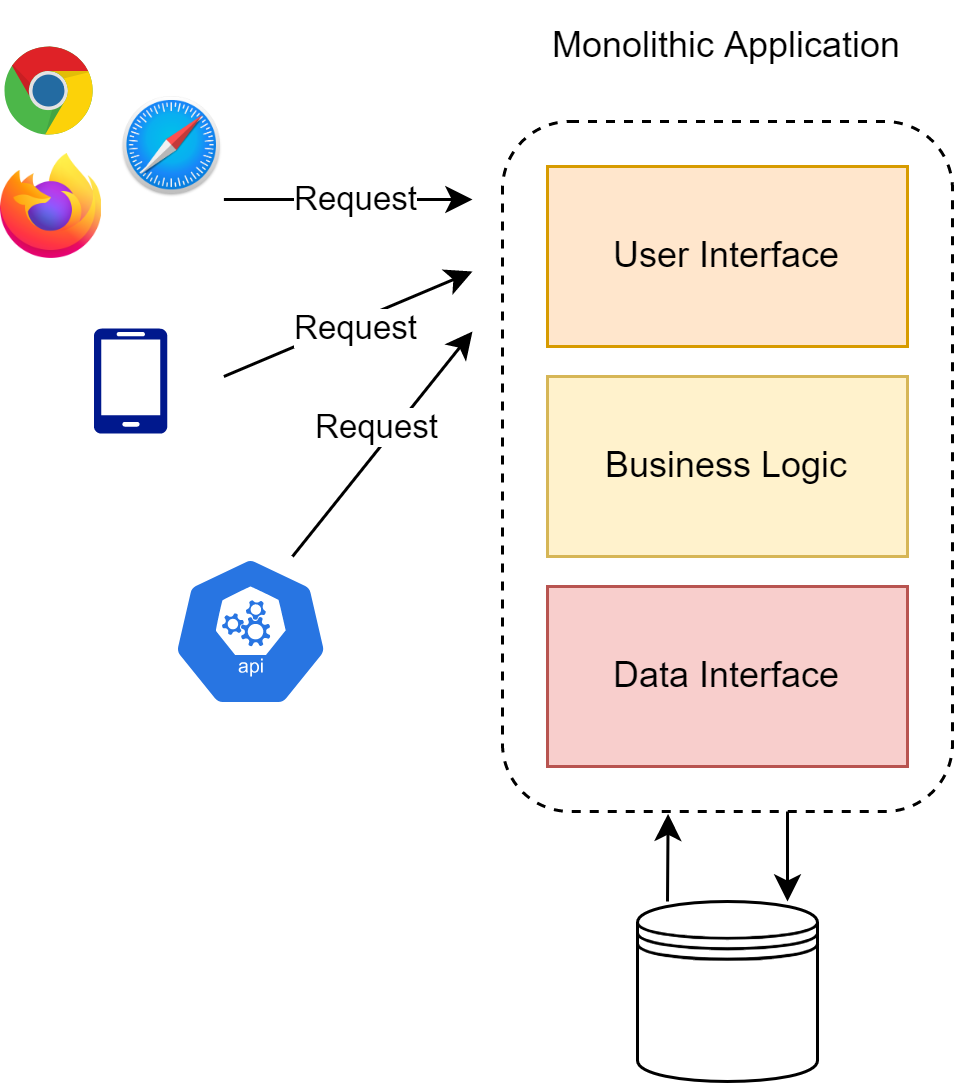
\includegraphics[width=0.7\linewidth]{img/Monolith.png}
 \end{center}
 \caption{Monolithic Architecture}
 \label{monolith}
\end{figure}

\noindent
A monolithic application has all services and business logic in one code base as displayed in Figure \ref{monolith}. The development team need to ensure when modifying services that other parts of the application do not break. Monolithic architectures are common in many applications due to their simplicity and ability to meet system requirements quickly while limiting the number of dependencies that must be satisfied at deployment time. For example, e-commerce applications tend to use monolithic architectures because they are relatively simple and can be deployed quickly to accelerate the time to market \cite{frommonotomicro}. However, as the system scales, the system becomes increasingly complex to maintain and troubleshoot. Dependency management becomes increasingly difficult, and managing releases becomes challenging as changes have to be made across multiple layers in the system. A monolithic architecture also introduces a single point of failure that can adversely impact the entire system if it fails \cite{vil2015}.

%//TODO: explain more

\section{Microservice}
\begin{figure} [H]
 \begin{center}
    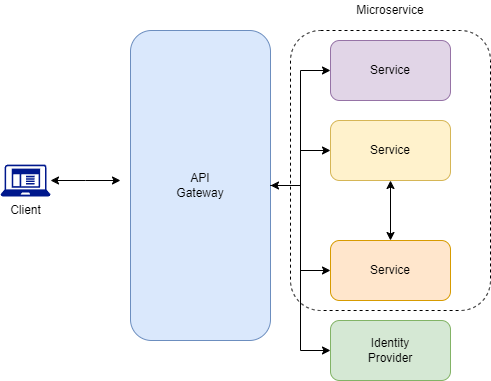
\includegraphics[width=1\linewidth]{img/Microservice_2.png}
 \end{center}
 \caption{Microservice Architecture}
 \label{microservice}
\end{figure}

\noindent
Microservices are an architectural style for building applications where each service performs a specific function and communicates with other services using asynchronous messaging. Each service typically exposes only a small set of its functionality via a web \ac{API}. Microservices can bring benefits, but they also pose challenges, especially regarding security aspects such as authentication and authorization \cite{alm2022} . There are also challenges related to the delivery, deployment, governance, and interoperability of services when migrating from a \ac{SOA} to microservices \cite{raj2021} . Researchers are exploring solutions to these challenges, such as the use of hybrid design patterns to promote resiliency and the enhancement of the saga pattern to resolve the lack of isolation issue \cite{ras2022, dar2022} .
\\
\\
Microservices are often built using \ac{API}-first approaches, where the \ac{API} is designed and developed first, followed by the other services that use it. This approach enables developers to prototype and test the microservices in isolation before integrating them into the main application, making development and testing faster and more cost-effective \cite{alm2022} . Once a service is successfully deployed, it can be used in other contexts where it may be used to achieve additional benefits. The microservice architecture also enables selecting the technology stack per service, allowing for greater flexibility and scalability \cite{dar2022} . However, the microservice architecture poses challenges, especially regarding security aspects such as authentication and authorization. Researchers are exploring solutions to these challenges, such as the use of \ac{JWT} \cite{alm2022} .
\\
\\
Microservices are a recent trend where each service can be developed, tested and scaled independently, making it much faster to develop and deploy new versions or features with minimal downtime for users. On the other hand, a monolithic \ac{API} approach is easier to maintain since it consists of a single process across the server instead of multiple processes that have to communicate over the network with each other \cite{pat2021}.

\section{Monolith vs Microservice} \label{movsmi}
\begin{table}[!h]
    \centering
    \begin{tabular}{|p{0.15\linewidth}|p{0.3\linewidth}|p{0.4\linewidth}|}
    \hline
        \textbf{Topic} & \textbf{Monolith} & \textbf{Microservice} \\ \hline
        Design & single code base & independent software components compiling and running autonomous \\ \hline
        Development & simple at the start, but more complex thus harder to maintain over time & more planning and infrastructure needed at the start, but easier to maintain over time \\ \hline
        Modification & change bears greater risk since it impacts the entire code base & modifying a single microservice does not impact the other microservices \\ \hline
        Debugging & code and bugs in the same environment & needs advanced debugging tool to trace stacktrace through potentially multiple microservices \\ \hline
        Deployment & app deployed as single unit & every microservice needs to be deployed independently \\ \hline
        Scale & need to scale entire app & can scale individual microservices \\ \hline
    \end{tabular}
    \caption{Comparison between Monolithic Architecture and Microservice Architecture}
\end{table}

\section{The Cloud}
By implementing DevOps practices in their organisations, companies can align IT operations with business goals and increase operational efficiency and agility. This is achieved by adopting new technologies like cloud computing, containerisation, microservices, and automation tools to speed up the development lifecycle and deliver high-quality products faster. Companies can for example reduce costs by renting IT infrastructure to support temporary required compute power \cite{qia2009}.

\subsection{\ac{IaaS}}
\ac{IaaS} solutions enable companies to build and deploy their own custom IT systems on the cloud without having to purchase and maintain any hardware or software. It enables them to focus on building their applications and business processes without worrying about the technical details related to the IT infrastructure. \ac{IaaS} also offers a lot of flexibility in terms of scaling up or down the resources required for their workloads as and when needed. It is still required to manage the OS and the package's whole deployment process.
\\
\\
Cloud providers such as AWS, Microsoft Azure, Google Cloud Platform, IBM Cloud, or Oracle Cloud provide cloud \ac{IaaS} that allows businesses to set up virtual machines on a shared infrastructure to manage their applications and workloads. \ac{IaaS} is a cloud service that provides virtualised computing resources (e.g. CPU, memory, storage and networking resources) on demand to users over the Internet. It is managed by the service provider using a cloud computing stack that consists of the underlying hardware, virtualisation software and the cloud management platform \cite{buy2019} .


\subsection{\ac{PaaS}}
\ac{PaaS} is a cloud computing service that provides a platform for developers to build and deploy their applications without worrying about the underlying infrastructure or hardware resources. So the differences to \ac{IaaS} is that with \ac{PaaS} users do not have to worry about the underlying infrastructure.
\\
\\
The main benefits of using \ac{PaaS} include the following:

\begin{itemize}
\item Quick Setup and Deployment: With \ac{PaaS}, developers no longer need to concern themselves with setting up and maintaining an IT infrastructure for running their applications, as all of this is done for them by the service provider. They can simply sign up for the service and start developing their application immediately and deploy it to the production environment by simply pushing a button without any further configuration or maintenance required. This can save a lot of time and effort on the developer's part so that they can focus on developing the application rather than troubleshooting technical issues \cite{law2008}.

\item Cost Effective: The acquisition and management of expensive hardware and software resources for running applications are no longer essential with the availability of cloud services. These services can significantly reduce the costs involved in maintaining such resources, which makes it a more cost-efficient alternative for organizations. Moreover, developers can utilize this platform in creating their software without requiring substantial infrastructure investments. \cite{gai2014}.

\item High Availability: To achieve high availability of applications and reduce costs, it is beneficial to scale them up or down depending on the required load. With this service, users can conveniently adjust their applications to match current workloads and thereby enjoy improved efficiency. They can easily downsize when the application is not needed, and upscale when a surge in demand occurs without additional costs. Moreover, the service accommodates diverse business requirements such as user analytics, data storage needs and available bandwidth. By utilising this method, developers can enhance the operation and capability of their software with regards to varying categories of consumers\cite{IaasHigh}.

\item Scalability: \ac{PaaS} allows developers to easily scale their applications to accommodate growing workload requirements without making additional investments \cite{law2008}. This is mainly achieved by integrating added resources that can be scaled up along with the workloads. Conversely, scaling down is equally straightforward when operational costs reduction and minimizing storage requirements are deemed necessary.
\end{itemize}


\section{Docker}
Docker is an open-source platform designed to automate application containers on a primarily Linux-based operating system. A Docker Container is lightweight, portable and isolated application packaging; developers can package an application and all its dependencies into a single file, known as a "container", that runs anywhere. Multiple containers may also be clustered together under one namespace allowing multiple processes running independently to share namespaces if needed. In addition, these lightweight files can easily move between development environments and production environments and be linked together into powerful apps \cite{rad2017}.
\\
\\
The key benefits of using Docker Containers include the following:

\begin{itemize}
\item Lightweight: Docker containers are generally smaller compared to a virtual machine. This means multiple applications can run on a single server without compromising performance \cite{vmwcovsvm}.

\item Portable: Docker containers are highly portable, which facilitates moving applications from development to production or even between different servers \cite{rad2017}. This is especially useful for DevOps teams as they can use the same containers in different environments, such as development and staging or production and testing.

\item Isolated: Docker containers are completely independent from one another on a system, reducing risk for vulnerabilities to affect multiple containers at once \cite{com2016}. Furthermore, this approach also makes it much easier to have multiple versions of runtimes or compilers installed - something virtual machines could make much harder to manage.

\item Easy to Manage: Docker containers are designed to minimise management overhead so developers can focus on building great apps instead of managing infrastructure. This is achieved by giving the developer fine-grained control over container resources and providing simple tools for managing them \cite{rad2017}.

\item Easily Scaled: As containers run on the Linux kernel, they are highly scalable and customisable - which enables them to meet diverse performance and resource requirements easily \cite{rad2017}. They also support most standard networking and storage technologies allowing deployment in any environment.
\end{itemize}

\noindent
Due to these advantages, Docker containers have quickly become the industry standard for deploying and running applications on public cloud services, making Docker containers widely adopted by both individual developers as well as large enterprises for all of their development and deployment needs.

\section{Kubernetes}
Kubernetes is open-source software for automating deployment, scaling and managing containerised applications. It provides a scalable way to run containerised applications on any public cloud or on-premise infrastructure. Kubernetes is workload agnostic, meaning that it can support multiple types of services without requiring the developers to re-architect the application for Kubernetes \cite{luk2018}.
\\
\\
Kubernetes features include resource provisioning, scalability, load balancing, service discovery, auto-scaling, etc. It also provides a Web \ac{API} for managing resources and a web-based dashboard for end users to monitor the status of the cluster and the resources in it. These features enable Kubernetes to control and monitor many containers simultaneously in a dynamic environment. It can also be used for development and testing environments as it can dynamically scale resources to meet user demand without deploying new servers each time additional resources are required \cite{kubernetes}.



\section{.NET Core}
.NET Core is a free, open-source, cross-platform development platform maintained by Microsoft \cite{dotnetintro}. It is a new version of the .NET Framework and is built on a high-performance platform \cite{dotnetintro}. It allows developers to build and run applications on Windows, Linux, and macOS.

\subsection{ASP.NET Core}
ASP.NET Core is an open source web application framework with wich one can write server-rendered web applications, web \ac{API}s and more. ASP.NET Core runs on Windows, Linux, macOS, and Docker \cite{Bobrov_2023}. Multiple versions of ASP.NET Core can exist side by side on the same server, meaning one app can adopt the latest version while other apps keep running on the version they were tested on \cite{dotnetaspcore}.
\\
\\
ASP.NET Core is used for developing professional web applications. It enables developers to construct modern, cross-platform apps using .NET Core technology. Solution architecture in ASP.Net Core can also accommodate for multi-domain management within one technical solution, thus serving multiple domains within an organization with one streamlined technical solution. This solution incorporates multiple design patterns such as Repository, Unit of Work and Inversion of Controls to address common developer problems while increasing business productivity. Furthermore, ASP.NET Core is used for web \ac{API} development; additionally organic benchmarks were set up between Java EE and ASP.NET Core runtimes to evaluate performance characteristics; Kestrel web server was employed to implement its version of the solution for ASP.NET Core implementation \cite{kro2018}.

\section{Web \ac{API}}
Web \ac{API} is a set of protocols and tools used for the creation of software applications. It outlines how software components should interact and enables communication among various software systems. Web \ac{API}s allow access to data and functionality of an online service or app, enabling developers to integrate systems more easily as well as build new apps which interact with existing ones \cite{soh2015}.
\\
\\
Web \ac{API}s allow users to make data requests to servers and receive responses in specific formats like JSON or XML \cite{tan2016}. They are accessible using \ac{HTTP} requests from any programming language or platform supporting \ac{HTTP}, making Web \ac{API}s ideal for tasks such as retrieving, updating, and performing calculations.
\\
\\
Web \ac{API}s have become ubiquitous across industries, from e-commerce and social media to finance2. Furthermore, they're widely employed within the Internet of Things (IoT) to enable communication between devices and systems \cite{tan2016}. Web \ac{API}s play an essential role in developing modern web apps and services that interact seamlessly with one another while offering users a positive user experience.

\section{\ac{JWT}}
The \ac{JWT} is widely recognized as the de facto standard for securely transmitting data in the form of a JSON object between multiple parties. It provides a concise and self-contained way for exchanging information that is trustworthy due to its digital signature \cite{akanajwt}. \ac{JWT}s can be signed using either a secret HMAC algorithm or through RSA or ECDSA using a public/private key pair. These tokens are employed in various scenarios such as authorization, single sign-on, and data exchange \cite{oauthjwt}.
\\
\\
Authorization is one prevalent application where \ac{JWT}s hold significant importance. Once users successfully log into their accounts, subsequent requests carry the \ac{JWT} token allowing them access to authorized routes, services, and resources associated with that specific token. Another noteworthy functionality heavily reliant upon \ac{JWT}s is single sign-on since these tokens possess minimal overhead and offer seamless integration across different domains \cite{jwt, oauthjwt}.
\\
\\
Comprised typically of three components - header, payload, and signature - each part plays an essential role within the architecture of \ac{JWT}s. The header delineates which cryptographic algorithm was employed in generating the signature whereas the payload encompasses claims or pertinent information encapsulated within a JSON object format \cite{superjwt}.

\section{Database}
A database is used for storing, fetching and manipulating data. There are multiple types of databases which dictate the structure of the data model. The two biggest distinctions are between relational and non-relational databases. This thesis uses Microsoft SQL Server which is a relational database \cite{whatmsSQLdb}, meaning it has a relational model which consists of a collection of tables which are made out of rows, columns and could potentially have relations \cite{oraclereldb, ibmreldb}.

\section{Swagger}
Swagger is an open-source set of rules, specifications, and tools for developing and documenting Web \ac{API}s. It enables developers to easily create interactive machine- and human-readable \ac{API} documentation. Swagger also offers an editor for OpenAPI specification files to generate interactive \ac{API} documentation quickly \cite{javapoint}. Furthermore, Swagger was built around OpenAPI spec files, consisting of three components - Swagger Editor, Swagger UI, and Codegen.
\\
\\
The Swagger Editor is a browser-based editor where developers can write and edit \ac{API} documentation and OpenAPI specifications. It can be used directly through the browser, downloaded to run locally, or used as part of SwaggerHub \cite{hubspot}. Similarly, Swagger UI generates interactive documentation from OpenAPI specifications, enabling users to visualize and interact with its resources without having any of its implementation logic in place. Lastly, Swagger Codegen generates server stubs and client libraries for \ac{API}s across many programming languages \cite{swagger}.
\\
\\
Swagger allows users to build, document, test and consume web services. It supports both top-down and bottom-up approaches for \ac{API} development; with top-down, or design-first approaches developers can design an \ac{API} prior to writing any code; while with bottom-up or code-first approaches Swagger takes the code written for an \ac{API} and generates its documentation. Standardizing \ac{API} writing processes with Swagger helps keep track of things which should ideally be included when designing \ac{API}s from scratch \cite{scaleyourapp}.

\section{Load Testing}
Load Testing is used to place a load on an application to ensure the application can handle the sudden influx of requests and remain stable. Load testing can be achieved through repeated, simultaneous requests. It reveals  possible software design flaws or bottlenecks within the application \cite{loadtest}.
\subsection{k6}
K6 is an load testing tool which helps with performance testing Web \ac{API}s and other Interfaces \cite{k6doc}. K6 is going to be used to load test the monolith and microservice.

\clearpage
%%%%%%%%%%%%%%%%%%%%%%%%%%%%   TODO: Applied Methods  %%%%%%%%%%%%%%%%%%%%%%%%%%%%
\chapter{Applied Methods}
The project created for this thesis called "Examich" is for students to create, manage and share practice exams. This service also offers the option to generate a PDF Version of the practice exams which will simulate a resource intensive action. Since this thesis focuses on the \ac{API} the frontend for this project will be skipped. The application was written as a monolith and then broken down into three microsercvices. The following sections will present how both version was implemented and how those were load tested.

\section{General Overlap}
Since the Microservice was created by splitting the Monolith many aspects of the projects remained the same so to not list those facts twice this section will present the similarities.
\\
\noindent
Both projects were written in C\# using .NET 5 utilising the QuestPDF library for generating the PDFs and storing data in the Microsoft SQL Server 2019. \ac{JWT} was used in both projects to handle authentication. Both the monolith and microservice are going to be deployed on Microsofts Cloud Service Azure Kubernetes.

\section{Monolith}
The following subsections will describe the architecture of the Monolith and outline the implementation.

\subsection{Architecture \& Implementation}
The monolith consists of three main parts as shown in Figure \ref{examichMonolith}. The \ac{API} that exposes the functionality to its users. The business logic which handles basic Create, Read, Update and Delete operations and generates PDFs. The data interface which handles the communication with the database. A seed of data was defined in the data interface for later to be queried by the load test.

\begin{figure} [H]
 \begin{center}
    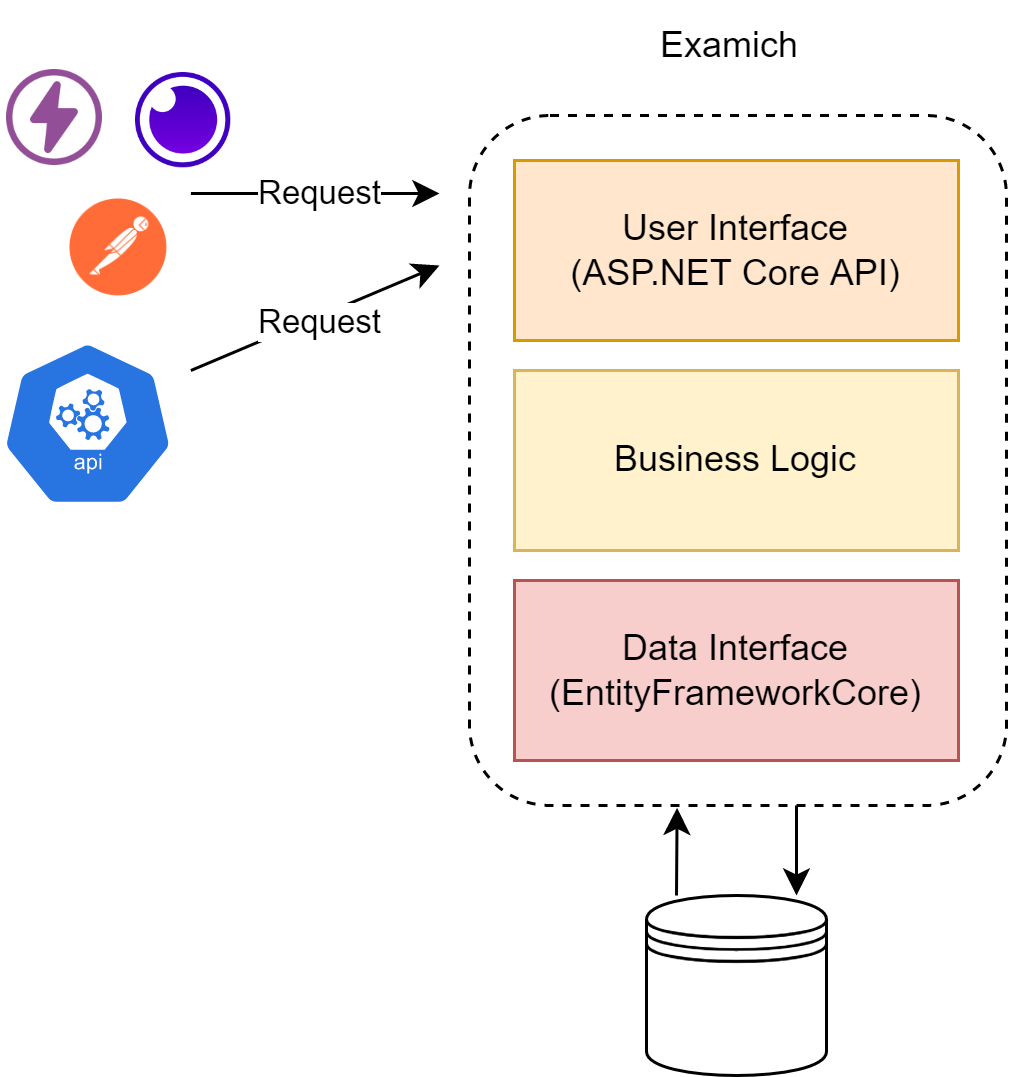
\includegraphics[width=0.6\linewidth]{img/ExamichMonolith.png}
 \end{center}
 \caption{Examich Monolith Architecture}
 \label{examichMonolith}
\end{figure}

\noindent
The monolith exposes the following web \ac{API} endpoints which will be load tested:

\begin{table}[!ht]
    \centering
    \begin{tabular}{|l|l|}
    \hline
        \ac{HTTP} Verb & URL \\ \hline
        POST & /api/Auth/Login \\ \hline
        GET & /api/Users/Search \\ \hline
        GET & /api/Exams/User \\ \hline
        GET & /api/Questions/Exam/\{examId\} \\ \hline
        GET & /api/Exams/\{examId\}/PDF \\ \hline
    \end{tabular}
 \caption{Relevant Examich Monolith Endpoints}
 \label{examichMonolithEndpoints}
\end{table}
\noindent
\\
The most resource intensive endpoint would be "/api/Exams/\{examId\}/PDF", since with this the PDF generation is triggered. It will render the PDF and send it as a response back to the user. The other endpoints are only for modifying data on the exams so mostly light on the resources.
\\
\\
\noindent
The application is packaged into a container image using a Dockerfile defining how to build the image which then will be used to create the container running the application. To deploy the application on Azure Kubernetes Cluster the structure must be defined in a YAML File. That YAML File defines the Image cluster should run is and on which port the application should be exposed.

\subsection{Data Model}

\begin{figure} [H]
 \begin{center}
    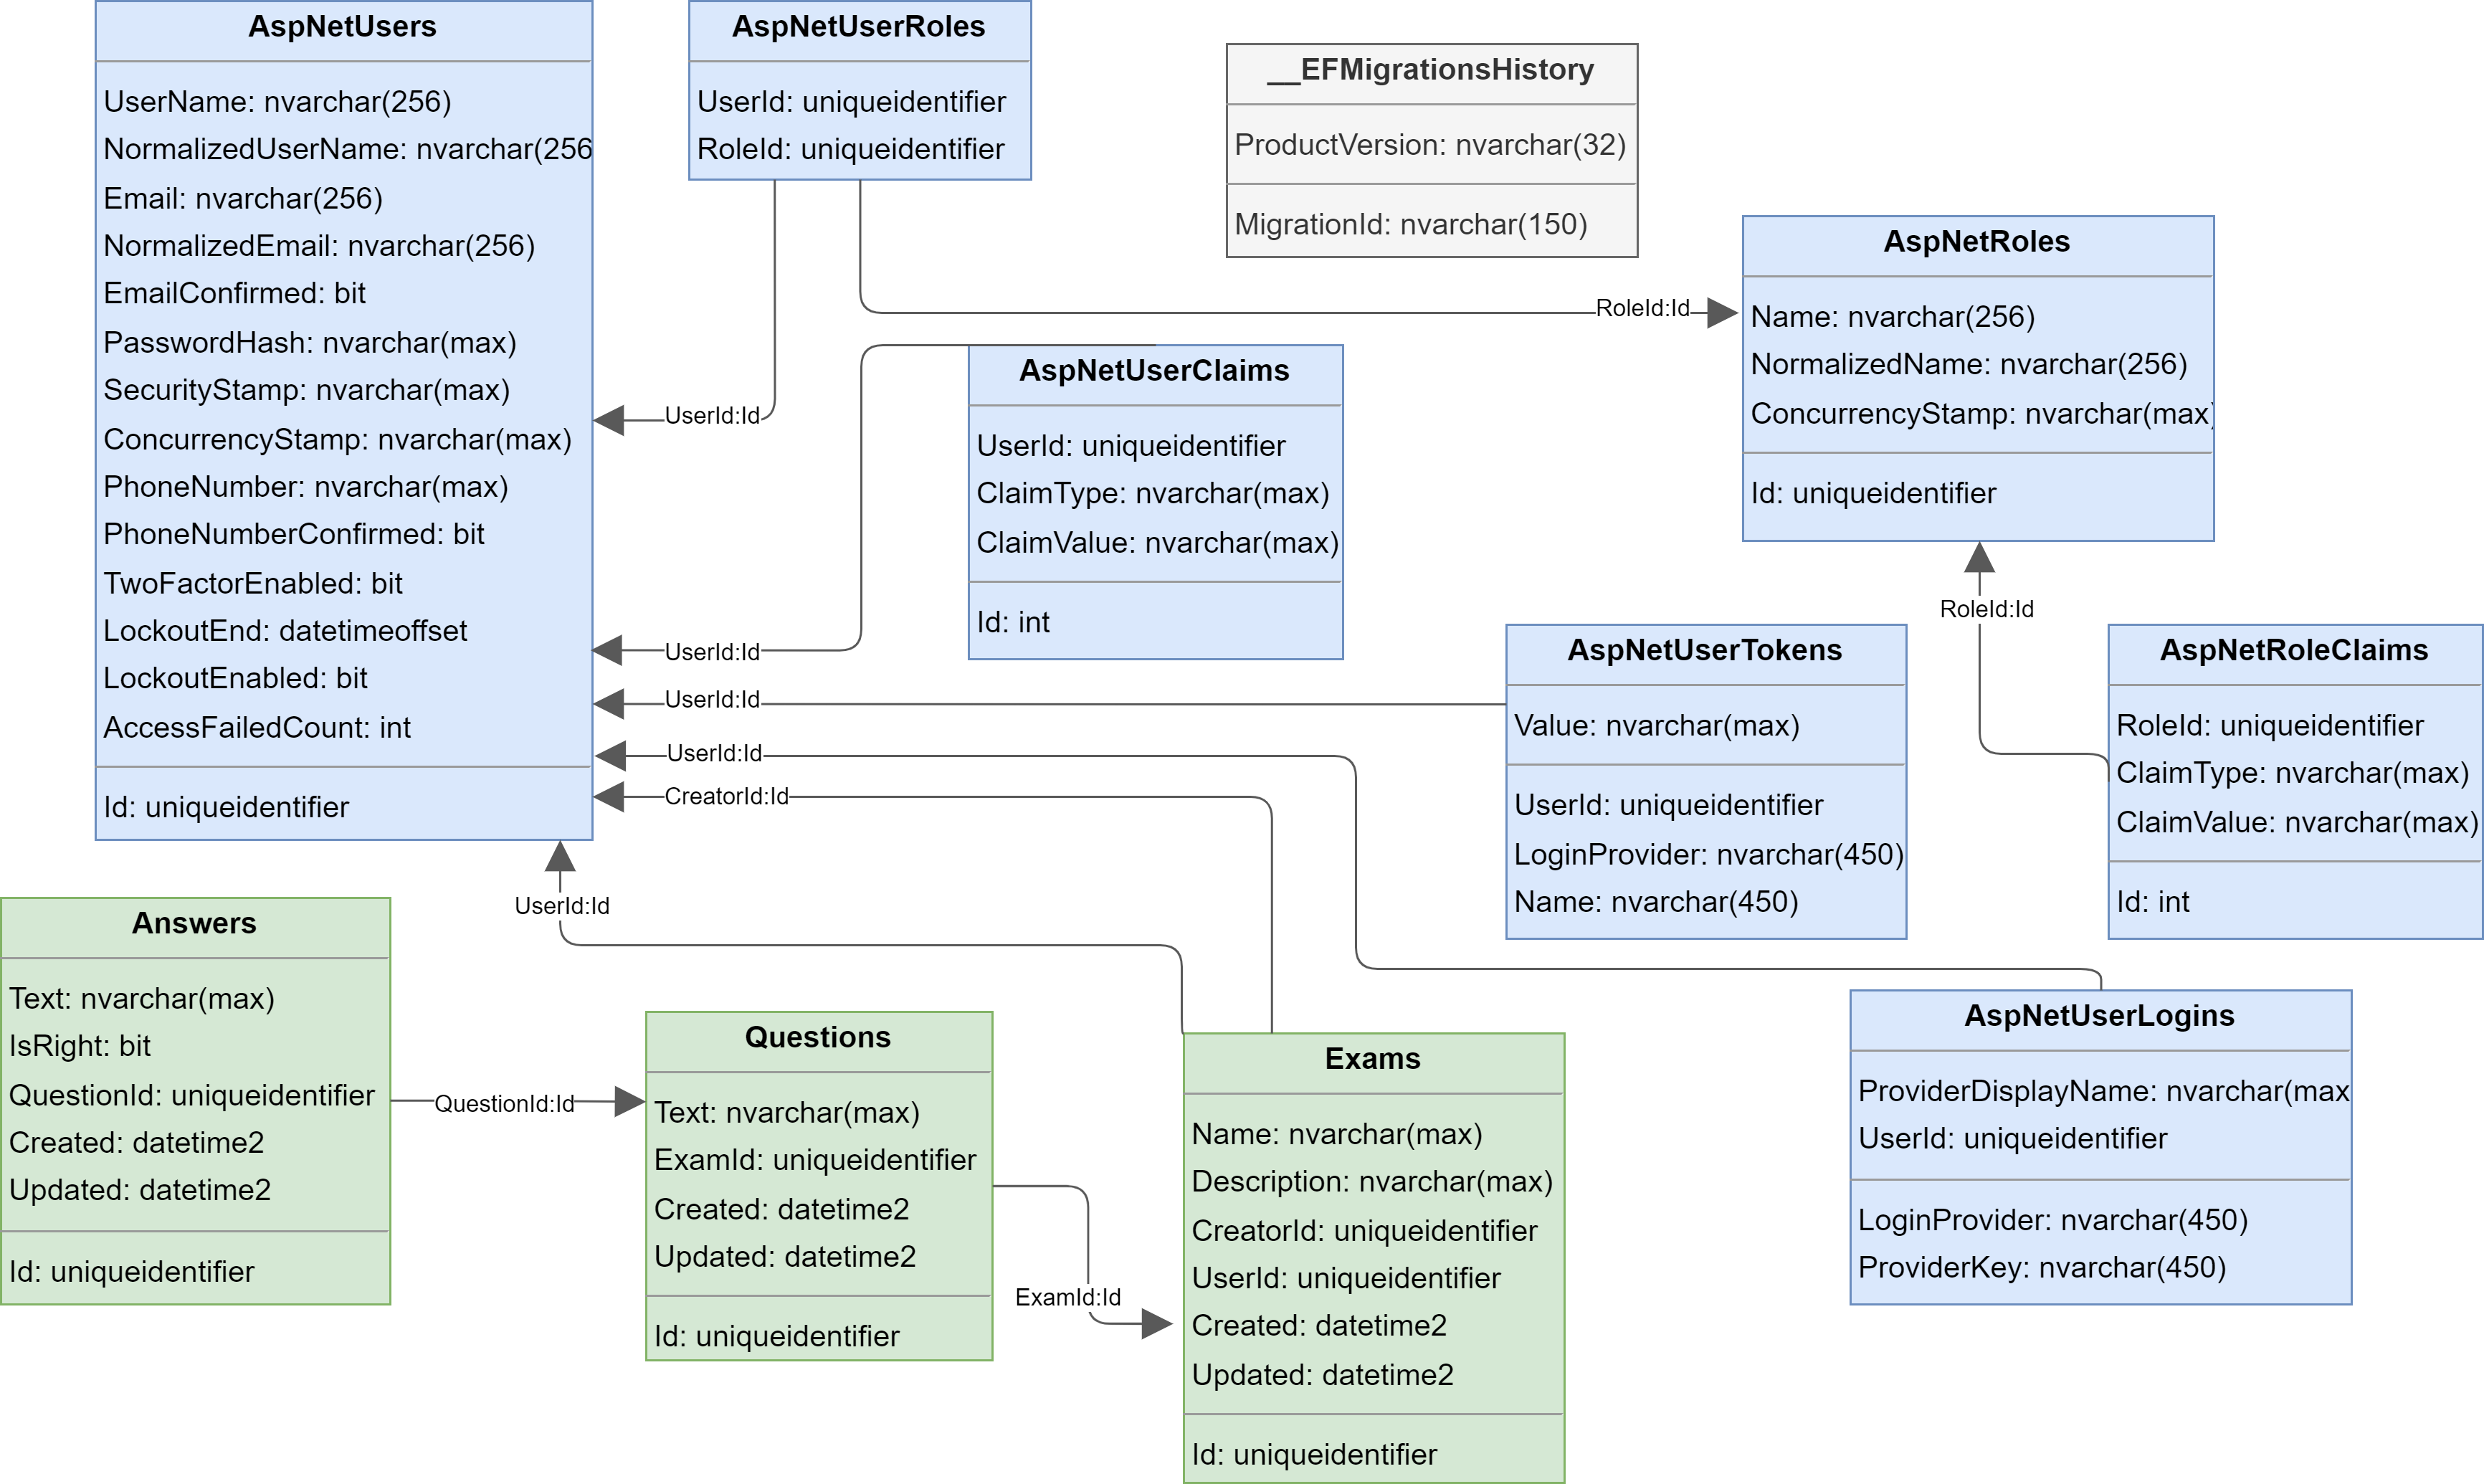
\includegraphics[width=1.1\linewidth]{img/ExamichDataModel.png}
 \end{center}
 \caption{Examich Monolith Data Model}
 \label{datamodel}
\end{figure}

Figure \ref{datamodel} presents the data model for the monolithic application. The blue tables are tables generated by Microsoft.AspNetCore.Identity.EntityFrameworkCore.IdentityDbContext used for user management and authentication, the grey one is generated by EntitiyFrameworkCore to keep track of the migrations and the green ones were specifically created for the project. Every User has zero or more Exams, every Exam has zero or more Questions and every Question has zero or more Answers.


\section{Microservice}
The following subsections will describe the architecture of the Microservice and outline the implementation.

\subsection{Architecture \& Implementation}
The Monolith was split into the three following Microservices as seen in Figure \ref{examichMicroservice}:

\begin{itemize}
\item User Service which handles, Login, Registration and queries regarding user data
\item Exam Service which handles, Create, Read, Update and Delete operations regarding Exams, Questions and Answers
\item PDF Service which handles generating a PDF out of one Exam
\end{itemize}
\begin{figure} [H]
 \begin{center}
    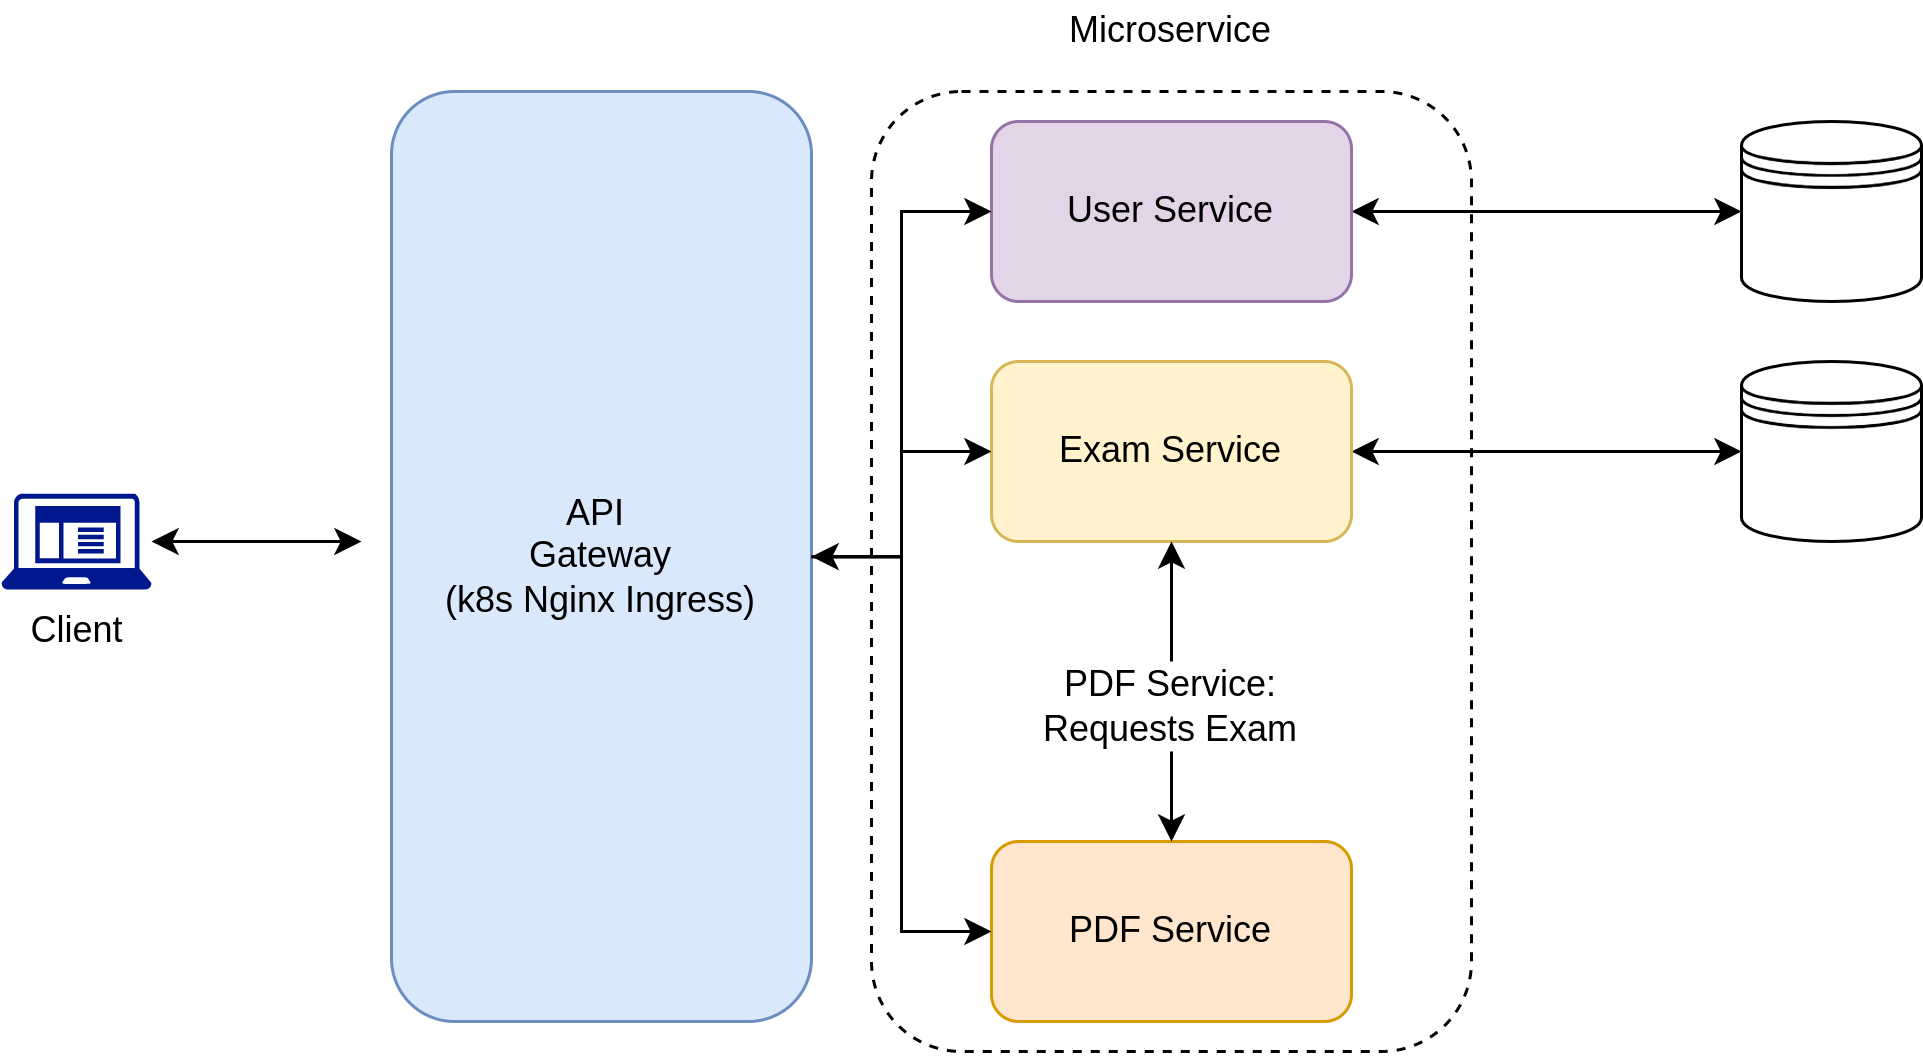
\includegraphics[width=1\linewidth]{img/ExamichMicroserviceArchitecture.png}
 \end{center}
 \caption{Examich Microservice Architecture}
 \label{examichMicroservice}
\end{figure}
\noindent
\\
All service are isolated and run independently from another, one service may still need the other. The User Service is completely isolated and also needs no other service to function as for the Exam Service. The PDF Service on the other hand needs data from the Exam Service to generate a PDF, so there is a dependency on the Exam Service. If the Exam Service is unavailable the PDF service would also fail but the User Service would still function. All endpoints remain the same as in Table \ref{examichMonolithEndpoints} except for the endpoint that handles the generating of the PDF which is under "/api/File/\{examId\}/PDF".
\\
\\
\noindent
The microservices like the monolith are packaged into container images and then deployed to the cluster with the differences that in the cluster there are now three Services. To expose those three services through the same Port  an Ingress is defined which forwards various routes to the appropriate Service.

\subsection{Data Model}
The Data Model for the Microservice is almost the same as for the Monolith in Figure \ref{datamodel} with the distinction that the data model was split in two. Two of the three services use a separate database with data only relevant to the service. Figure \ref{datamodelmicroservice} displays that split with one database used for the User Service including all User related tables and one database for the Exam Service including all Exam related tables.
\begin{figure} [H]
 \begin{center}
    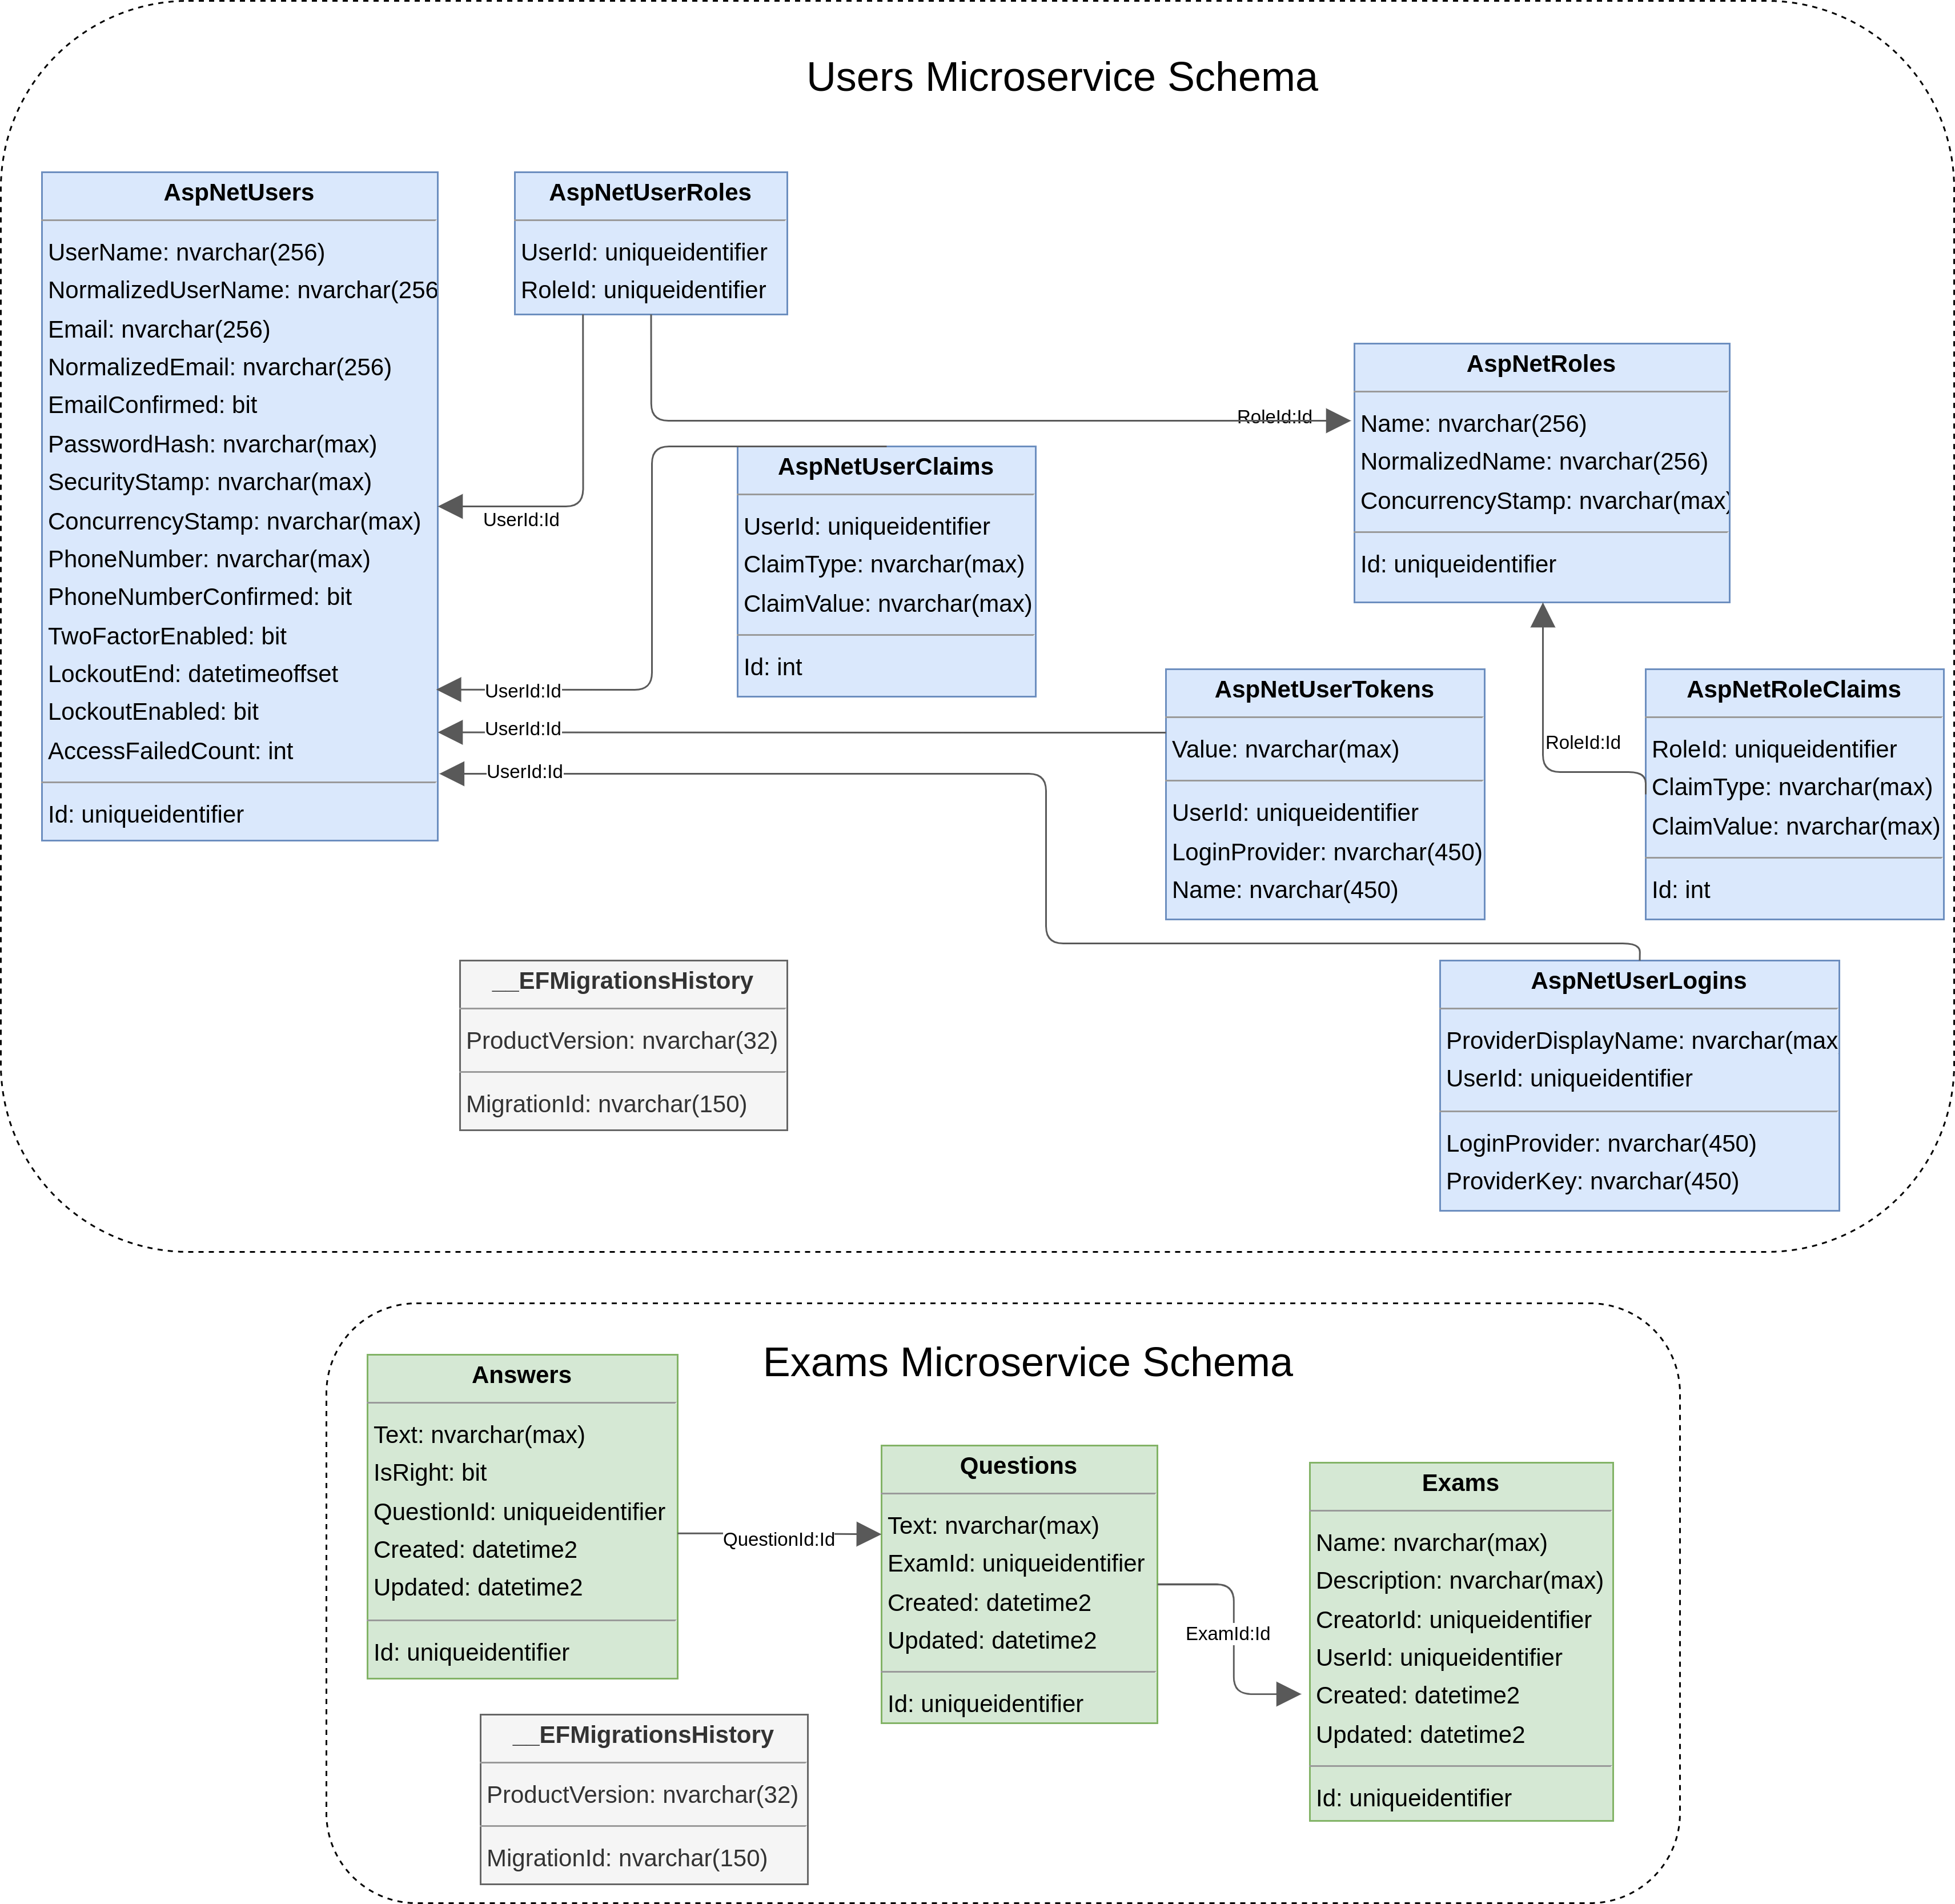
\includegraphics[width=1\linewidth]{img/ExamichMicroserviceDataModel.png}
 \end{center}
 \caption{Examich Microservice Data Model}
 \label{datamodelmicroservice}
\end{figure}

\section{Performance Benchmark}
This chapter will cover how the performance with k6 was executed and what measurements were taken. Load tests with k6 are simulated through \ac{VU}s which makes it very CPU intensive so a VM with many cores is needed. As mentioned in the previous section following endpoints of both applications are being tested:

\begin{table}[!ht]
    \centering
    \begin{tabular}{|l|l|}
    \hline
        \ac{HTTP} Verb & URL \\ \hline
        POST & /api/Auth/Login \\ \hline
        GET & /api/Users/Search \\ \hline
        GET & /api/Exams/User \\ \hline
        GET & /api/Questions/Exam/\{examId\} \\ \hline
        GET & (Monolith only) /api/Exams/\{examId\}/PDF \\ \hline
        GET & (Microservice only) /api/File/\{examId\}/PDF \\ \hline
    \end{tabular}
 \caption{Endpoints subject to load tests}
 \label{loadTestEndpoints}
\end{table}

\noindent
k6 will ramp up to 300 \ac{VU}s in one minute and after another minute take two minutes to ramp up to 900 \ac{VU}s in which k6 will remain for 3 minutes and then ramp down the same way it ramped down. The whole test needs 10 minutes per endpoint. To ensure low latency in the tests the k6 agent will run on an Azure Virtual Machine in the same Datacenter as the Azure Kubernetes Cluster. To set even grounds for the tests with the individual endpoints each service has four endpoints while the monolith also has only four containers.

\chapter{Discussion \& Results}
After executing the load tests the data compiled and visualized as graphs for this thesis are the total requests done in the 9 minutes per endpoint and the duration the request took. The duration consists of k6 sending the request, the time it waited for a response and the time until the full response was received. The DNS lookup and connection times regarding DNS are not taken into account.

\subsection{Light Resource Endpoints}
The following graphs are of lighter resource usage endpoints. The differences shown by these graphs between monolith and microservice are minimal and bearly distinguishable.


% #region login
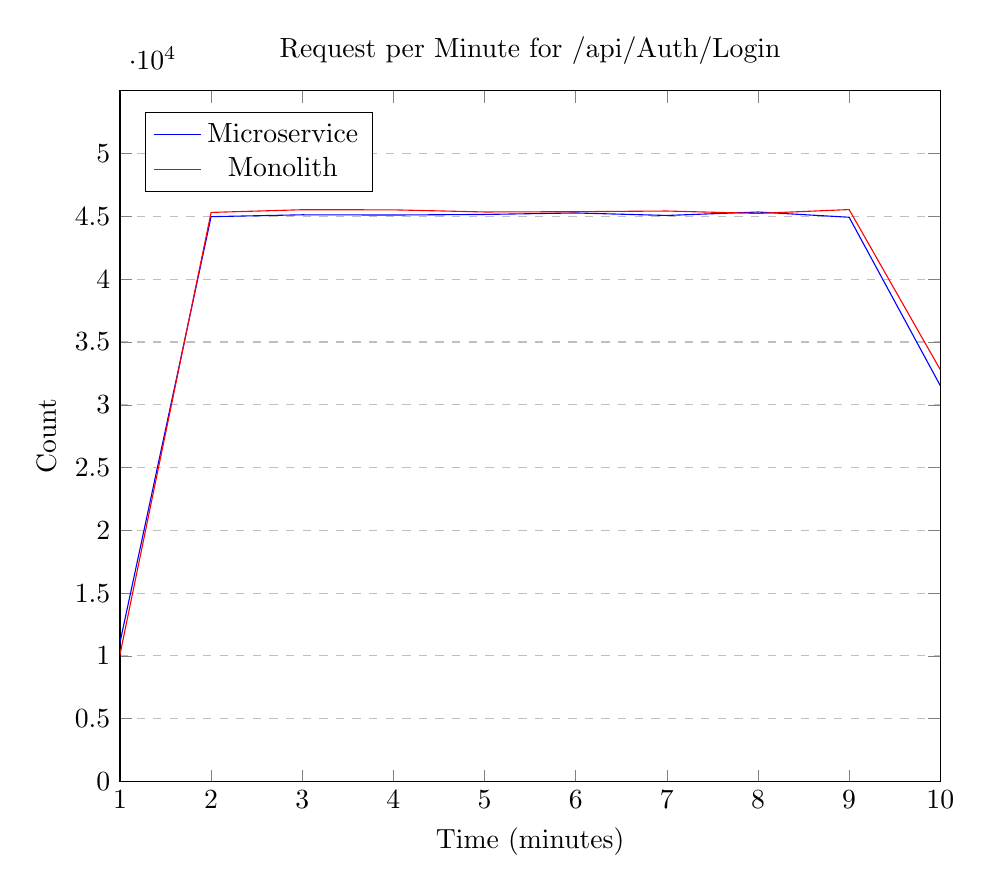
\begin{tikzpicture}
\begin{axis}[
    title={Request per Minute for /api/Auth/Login},
    xlabel={Time (minutes)},
    ylabel={Count},
    xmin=1, xmax=10,
    ymin=0, ymax=55000,
    xtick={1,2,3,4,5,6,7,8,9,10},
    ytick={0, 5000, 10000, 15000, 20000, 25000, 30000, 35000, 40000, 45000, 50000},
    legend pos=north west,
    ymajorgrids=true,
    grid style=dashed,
    width=12cm
]

\addplot[
    color=blue,
   %  mark=square,
    ]
    coordinates {(1, 11055)(2, 44985)(3, 45134)(4, 45116)(5, 45162)(6, 45281)(7, 45081)(8, 45355)(9, 44938)(10, 31527)
}; \addlegendentry{Microservice}

\addplot[
    color=red,
   %  mark=square,
    ]
    coordinates {(1, 10100)(2, 45323)(3, 45538)(4, 45529)(5, 45359)(6, 45381)(7, 45435)(8, 45243)(9, 45551)(10, 32794)
}; \addlegendentry{Monolith}

\end{axis}
\end{tikzpicture}
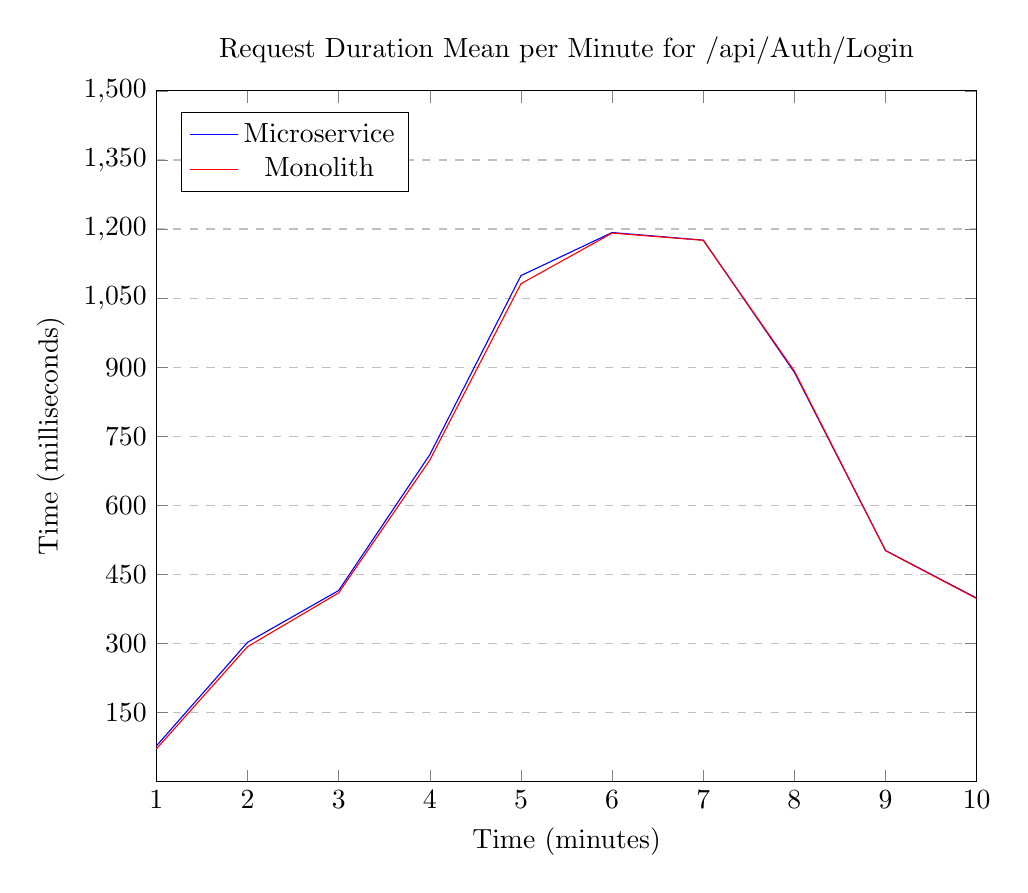
\begin{tikzpicture}
\begin{axis}[
    title={Request Duration Mean per Minute for /api/Auth/Login},
    xlabel={Time (minutes)},
    ylabel={Time (milliseconds)},
    xmin=1, xmax=10,
    ymin=0, ymax=1500,
    xtick={1,2,3,4,5,6,7,8,9,10},
    ytick={150, 300, 450, 600, 750, 900, 1050, 1200, 1350, 1500},
    legend pos=north west,
    ymajorgrids=true,
    grid style=dashed,
    width=12cm
]

\addplot[
    color=blue,
   %  mark=square,
    ]
    coordinates {(1, 76.96608583)(2, 302.0921593)(3, 414.7108936)(4, 709.851739)(5, 1098.846158)(6, 1192.401942)(7, 1175.931465)(8, 888.5370464)(9, 501.5327909)(10, 398.2923708)
}; \addlegendentry{Microservice}

\addplot[
    color=red,
   %  mark=square,
    ]
    coordinates {(1, 70.56194977)(2, 292.6783839)(3, 409.5729679)(4, 698.188539)(5, 1081.159473)(6, 1191.194963)(7, 1175.495195)(8, 891.3331957)(9, 501.1194849)(10, 397.0542417)
}; \addlegendentry{Monolith}

\end{axis}
\end{tikzpicture}
% endregion

% #region questions
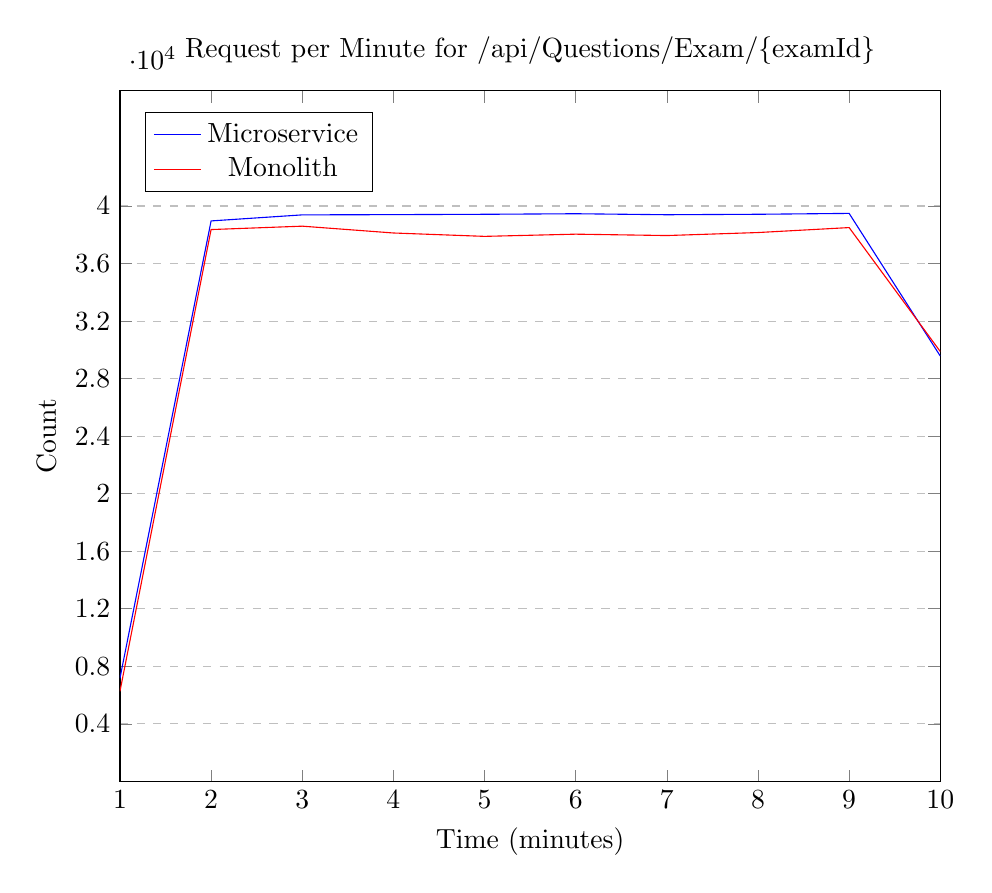
\begin{tikzpicture}
\begin{axis}[
    title={Request per Minute for /api/Questions/Exam/\{examId\}},
    xlabel={Time (minutes)},
    ylabel={Count},
    xmin=1, xmax=10,
    ymin=0, ymax=48000,
    xtick={1,2,3,4,5,6,7,8,9,10},
    ytick={4000, 8000, 12000, 16000, 20000, 24000, 28000, 32000, 36000, 40000},
    legend pos=north west,
    ymajorgrids=true,
    grid style=dashed,
    width=12cm
]

\addplot[
    color=blue,
   %  mark=square,
    ]
    coordinates {(1, 7172)(2, 38964)(3, 39384)(4, 39401)(5, 39425)(6, 39463)(7, 39394)(8, 39426)(9, 39487)(10, 29570)
}; \addlegendentry{Microservice}

\addplot[
    color=red,
   %  mark=square,
    ]
    coordinates {(1, 6256)(2, 38363)(3, 38599)(4, 38125)(5, 37890)(6, 38043)(7, 37947)(8, 38156)(9, 38501)(10, 29884)
}; \addlegendentry{Monolith}

\end{axis}
\end{tikzpicture}
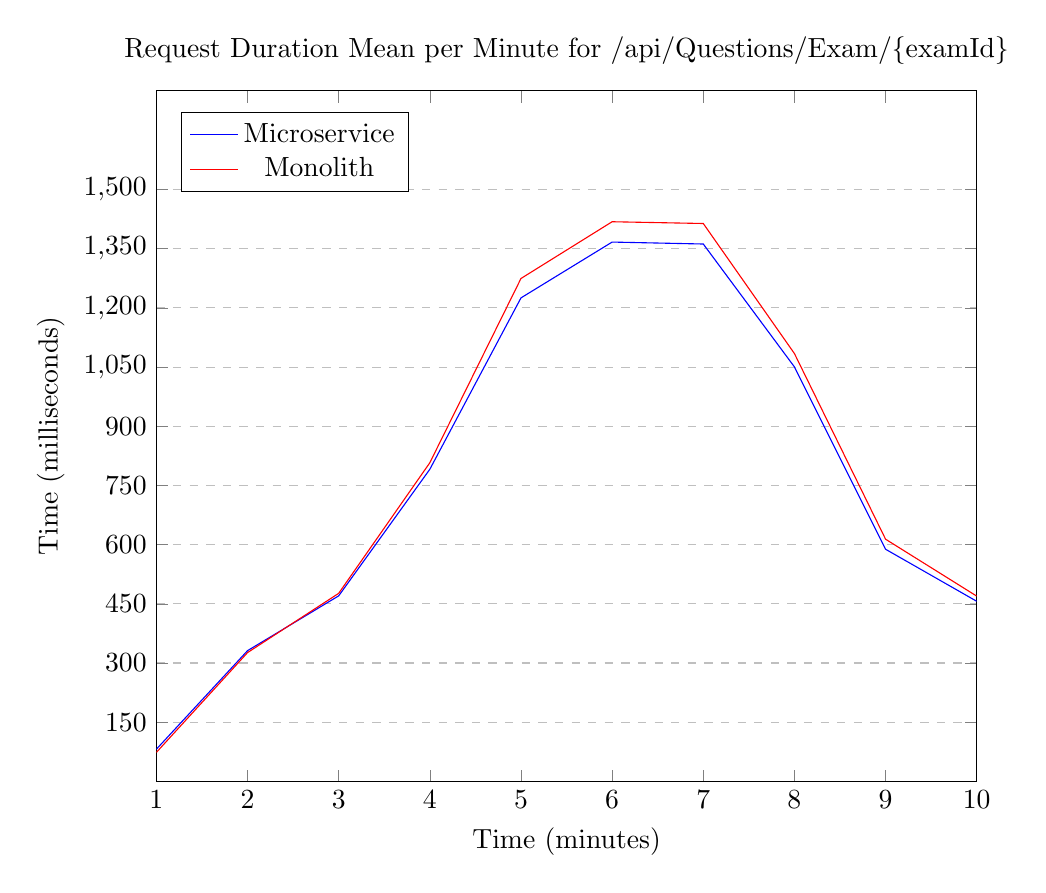
\begin{tikzpicture}
\begin{axis}[
    title={Request Duration Mean per Minute for /api/Questions/Exam/\{examId\}},
    xlabel={Time (minutes)},
    ylabel={Time (milliseconds)},
    xmin=1, xmax=10,
    ymin=0, ymax=1750,
    xtick={1,2,3,4,5,6,7,8,9,10},
    ytick={150, 300, 450, 600, 750, 900, 1050, 1200, 1350, 1500},
    legend pos=north west,
    ymajorgrids=true,
    grid style=dashed,
    width=12cm
]

\addplot[
    color=blue,
   %  mark=square,
    ]
    coordinates {(1, 81.57901054)(2, 331.3201321)(3, 470.2103125)(4, 791.0683888)(5, 1225.472245)(6, 1366.962076)(7, 1362.035365)(8, 1050.547978)(9, 588.4202396)(10, 456.4667852)
}; \addlegendentry{Microservice}

\addplot[
    color=red,
   %  mark=square,
    ]
    coordinates {(1, 73.50566628)(2, 326.3956512)(3, 476.6389503)(4, 807.632652)(5, 1274.649247)(6, 1418.484783)(7, 1414.013025)(8, 1084.419876)(9, 613.8820904)(10, 469.5884698)
}; \addlegendentry{Monolith}

\end{axis}
\end{tikzpicture}
% endregion

The duration and the amount of requests handled for both architectures are about the same showing that for web \ac{API} endpoints with low resource usage microservices do not bring any performance benefits in this case.

\clearpage
\subsection{Heavy Resource Endpoints}
The following graphs of endpoints with higher resource usage display the gap between monolith and microservice widening in favor of the microservice.



% #region users
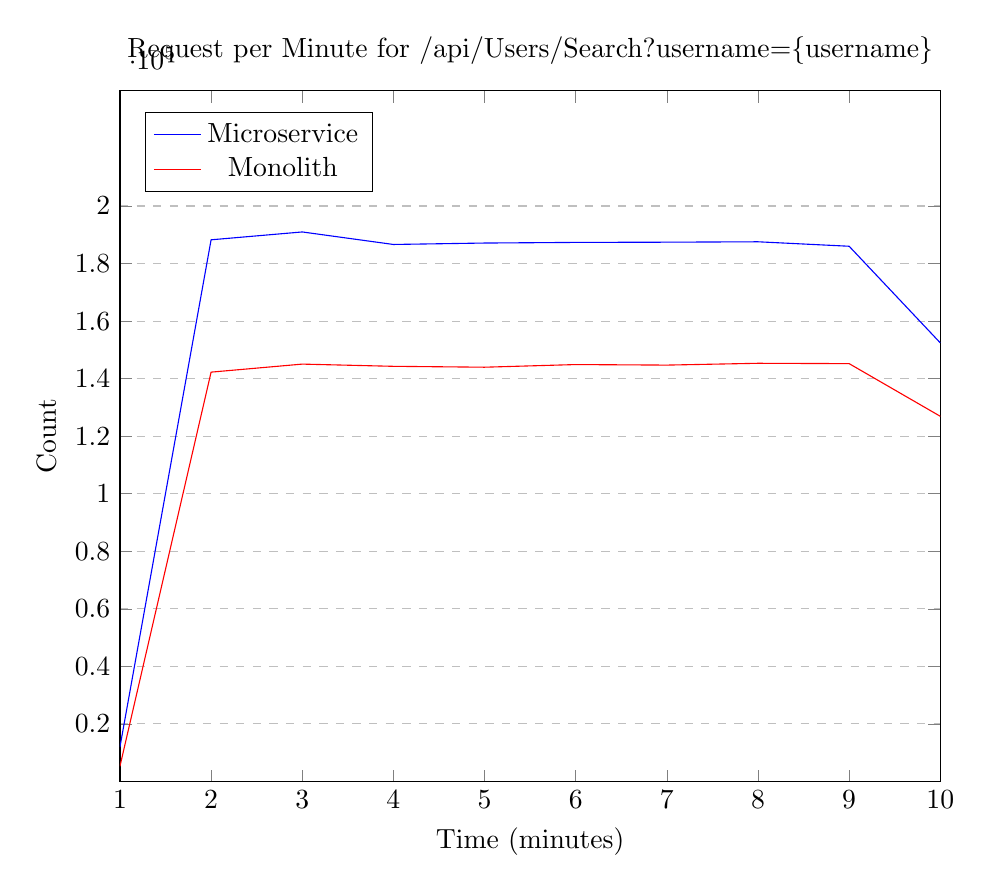
\begin{tikzpicture}
\begin{axis}[
    title={Request per Minute for /api/Users/Search?username=\{username\}},
    xlabel={Time (minutes)},
    ylabel={Count},
    xmin=1, xmax=10,
    ymin=0, ymax=240000,
    xtick={1,2,3,4,5,6,7,8,9,10},
    ytick={20000, 40000, 60000, 80000, 100000, 120000, 140000, 160000, 180000, 200000},
    legend pos=north west,
    ymajorgrids=true,
    grid style=dashed,
    width=12cm
]

\addplot[
    color=blue,
   %  mark=square,
    ]
    coordinates {(1, 11960)(2, 188256)(3, 190987)(4, 186635)(5, 187132)(6, 187351)(7, 187430)(8, 187568)(9, 186016)(10, 152433)
}; \addlegendentry{Microservice}

\addplot[
    color=red,
   %  mark=square,
    ]
    coordinates {(1, 5251)(2, 142260)(3, 145048)(4, 144279)(5, 143970)(6, 144891)(7, 144703)(8, 145334)(9, 145214)(10, 126912)
}; \addlegendentry{Monolith}

\end{axis}
\end{tikzpicture}
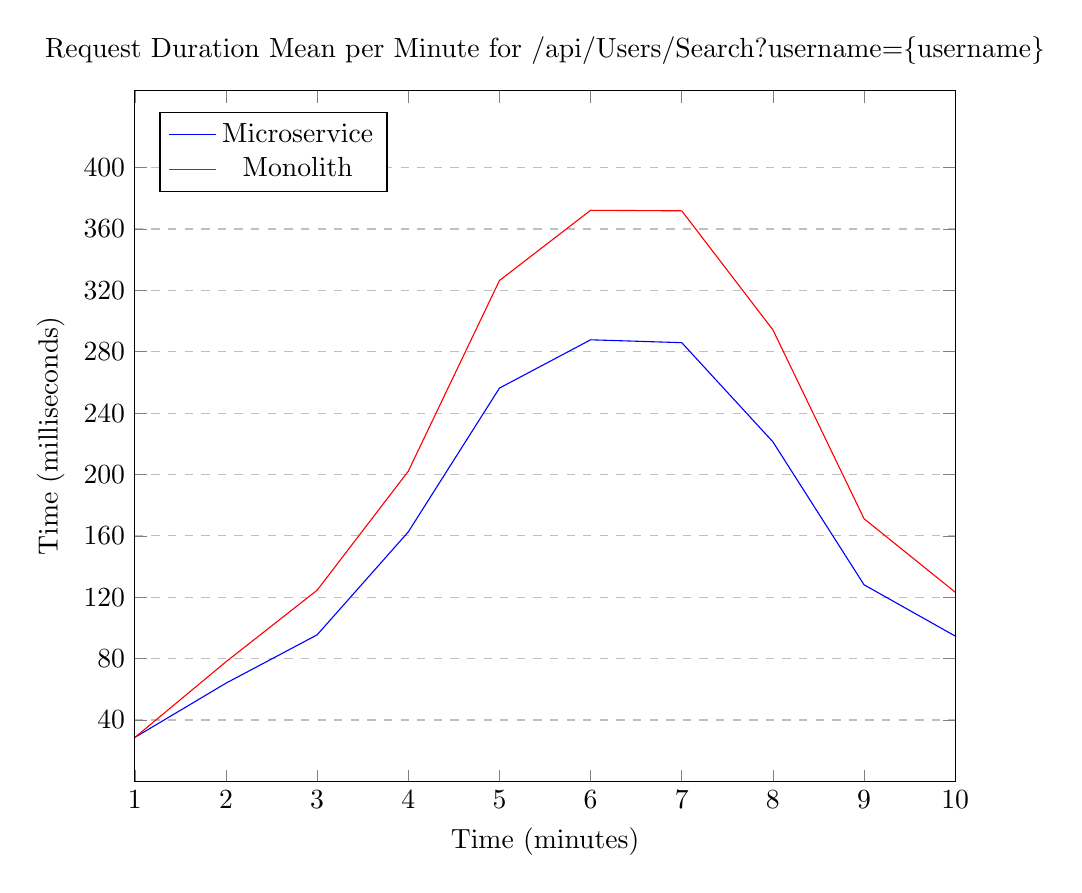
\begin{tikzpicture}
\begin{axis}[
    title={Request Duration Mean per Minute for /api/Users/Search?username=\{username\}},
    xlabel={Time (minutes)},
    ylabel={Time (milliseconds)},
    xmin=1, xmax=10,
    ymin=0, ymax=450,
    xtick={1,2,3,4,5,6,7,8,9,10},
    ytick={40, 80, 120, 160, 200, 240, 280, 320, 360, 400},
    legend pos=north west,
    ymajorgrids=true,
    grid style=dashed,
    width=12cm
]

\addplot[
    color=blue,
   %  mark=square,
    ]
    coordinates {(1, 28.64911701)(2, 64.01450185)(3, 95.51244705)(4, 162.6077447)(5, 256.3218017)(6, 287.8049417)(7, 285.9397712)(8, 221.3044419)(9, 128.1369566)(10, 94.71526498)
}; \addlegendentry{Microservice}

\addplot[
    color=red,
   %  mark=square,
    ]
    coordinates {(1, 28.62215946)(2, 77.96694228)(3, 124.6195747)(4, 202.1805984)(5, 326.4333459)(6, 372.2103948)(7, 371.8769494)(8, 294.295701)(9, 171.1912288)(10, 123.3112889)
}; \addlegendentry{Monolith}

\end{axis}
\end{tikzpicture}
% endregion



% #region exams
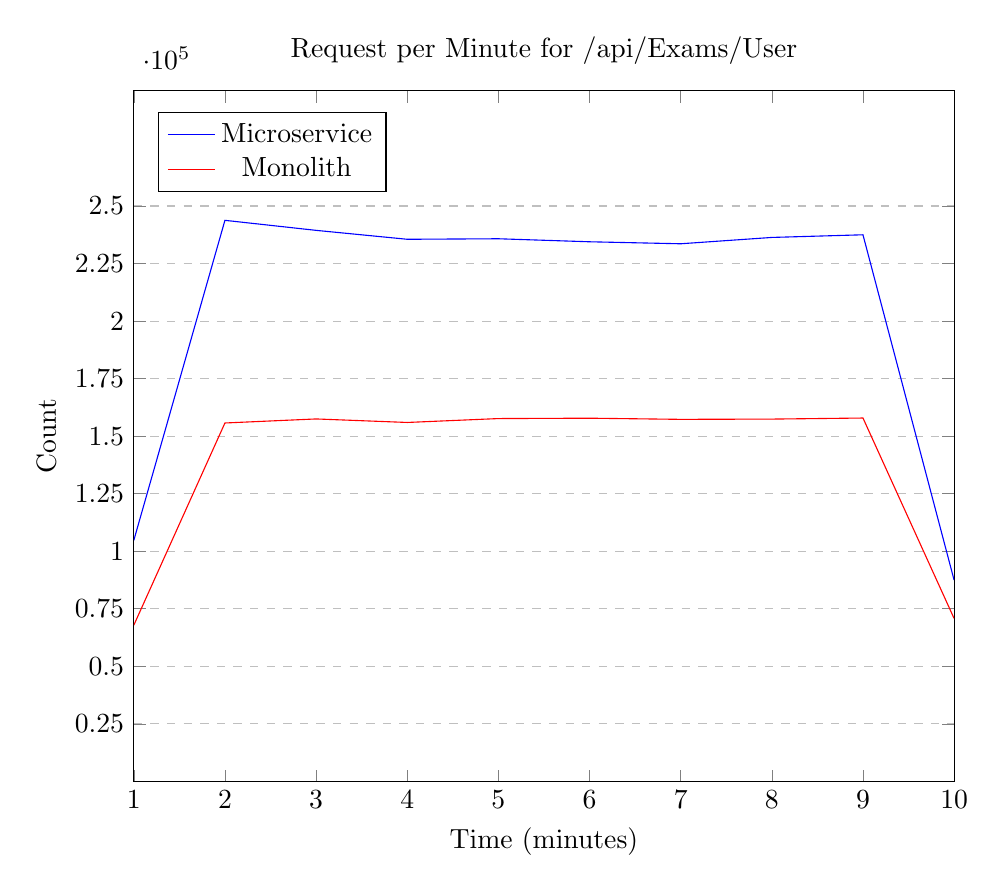
\begin{tikzpicture}
\begin{axis}[
    title={Request per Minute for /api/Exams/User},
    xlabel={Time (minutes)},
    ylabel={Count},
    xmin=1, xmax=10,
    ymin=0, ymax=300000,
    xtick={1,2,3,4,5,6,7,8,9,10},
    ytick={25000, 50000, 75000, 100000, 125000, 150000, 175000, 200000, 225000, 250000},
    legend pos=north west,
    ymajorgrids=true,
    grid style=dashed,
    width=12cm
]

\addplot[
    color=blue,
   %  mark=square,
    ]
    coordinates {(1, 104699)(2, 243780)(3, 239423)(4, 235549)(5, 235771)(6, 234462)(7, 233596)(8, 236347)(9, 237497)(10, 87437)
}; \addlegendentry{Microservice}

\addplot[
    color=red,
   %  mark=square,
    ]
    coordinates {(1, 67838)(2, 155723)(3, 157482)(4, 155952)(5, 157645)(6, 157806)(7, 157304)(8, 157418)(9, 157881)(10, 70778)
}; \addlegendentry{Monolith}

\end{axis}
\end{tikzpicture}
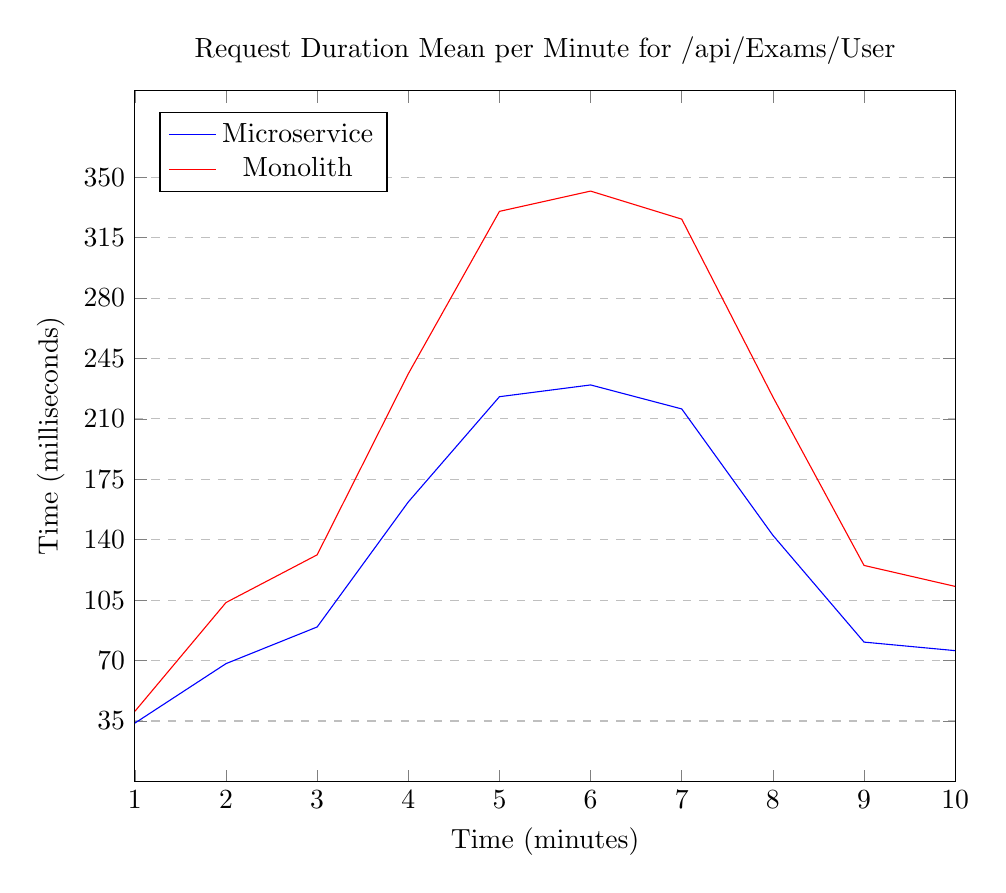
\begin{tikzpicture}
\begin{axis}[
    title={Request Duration Mean per Minute for /api/Exams/User},
    xlabel={Time (minutes)},
    ylabel={Time (milliseconds)},
    xmin=1, xmax=10,
    ymin=0, ymax=400,
    xtick={1,2,3,4,5,6,7,8,9,10},
    ytick={35, 70, 105, 140, 175, 210, 245, 280, 315, 350},
    legend pos=north west,
    ymajorgrids=true,
    grid style=dashed,
    width=12cm
]

\addplot[
    color=blue,
   %  mark=square,
    ]
    coordinates {(1, 33.75440701)(2, 68.22505615)(3, 89.45933764)(4, 161.8957117)(5, 222.8614944)(6, 229.6773783)(7, 215.7759879)(8, 142.5641189)(9, 80.69090542)(10, 75.74630315)
}; \addlegendentry{Microservice}

\addplot[
    color=red,
   %  mark=square,
    ]
    coordinates {(1, 40.57101134)(2, 103.6190858)(3, 131.2498636)(4, 236.1547766)(5, 330.2298651)(6, 341.9802514)(7, 325.7255893)(8, 222.7114201)(9, 125.1077236)(10, 112.9569517)
}; \addlegendentry{Monolith}

\end{axis}
\end{tikzpicture}
% endregion


% #region file
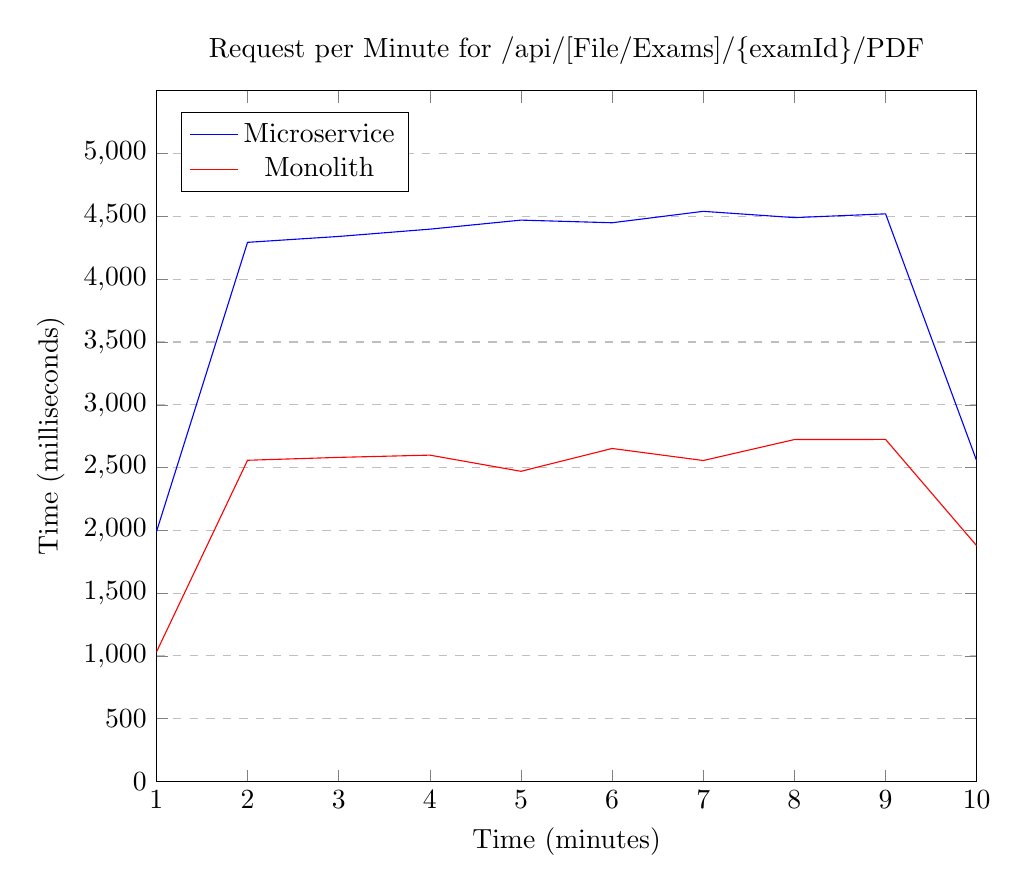
\begin{tikzpicture}
\begin{axis}[
    title={Request per Minute for /api/[File/Exams]/\{examId\}/PDF},
    xlabel={Time (minutes)},
    ylabel={Time (milliseconds)},
    xmin=1, xmax=10,
    ymin=0, ymax=5500,
    xtick={1,2,3,4,5,6,7,8,9,10},
    ytick={0,500, 1000, 1500, 2000, 2500, 3000, 3500, 4000, 4500, 5000},
    legend pos=north west,
    ymajorgrids=true,
    grid style=dashed,
    width=12cm
]

\addplot[
    color=blue,
   %  mark=square,
    ]
    coordinates {(1, 1987)(2, 4294)(3, 4341)(4, 4399)(5, 4471)(6, 4450)(7, 4541)(8, 4491)(9, 4521)(10, 2553)
}; \addlegendentry{Microservice}

\addplot[
    color=red,
   %  mark=square,
    ]
    coordinates {(1, 1029)(2, 2558)(3, 2581)(4, 2599)(5, 2470)(6, 2652)(7, 2556)(8, 2723)(9, 2724)(10, 1877)
}; \addlegendentry{Monolith}

\end{axis}
\end{tikzpicture}
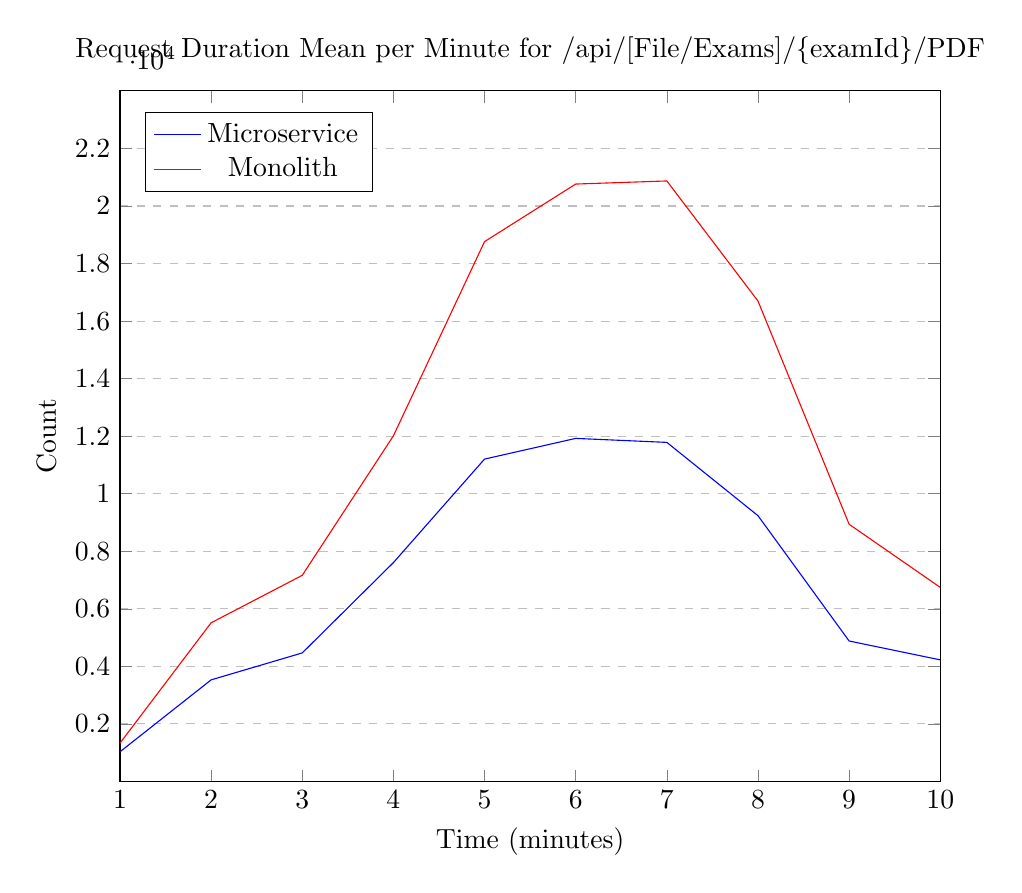
\begin{tikzpicture}
\begin{axis}[
    title={Request Duration Mean per Minute for /api/[File/Exams]/\{examId\}/PDF},
    xlabel={Time (minutes)},
    ylabel={Count},
    xmin=1, xmax=10,
    ymin=0, ymax=24000,
    xtick={1,2,3,4,5,6,7,8,9,10},
    ytick={2000, 4000, 6000, 8000, 10000, 12000, 14000, 16000, 18000, 20000, 22000},
    legend pos=north west,
    ymajorgrids=true,
    grid style=dashed,
    width=12cm
]

\addplot[
    color=blue,
   %  mark=square,
    ]
    coordinates {(1, 1027.690308)(2, 3528.517883)(3, 4465.213087)(4, 7604.881331)(5, 11202.96727)(6, 11922.4563)(7, 11783.95181)(8, 9236.021711)(9, 4879.770097)(10, 4223.731491)
}; \addlegendentry{Microservice}

\addplot[
    color=red,
   %  mark=square,
    ]
    coordinates {(1, 1327.496037)(2, 5512.226077)(3, 7162.583965)(4, 12011.17865)(5, 18762.64226)(6, 20763.42031)(7, 20871.45949)(8, 16697.1511)(9, 8937.347008)(10, 6742.616808)
}; \addlegendentry{Monolith}

\end{axis}
\end{tikzpicture}
% endregion


The duration and the amount of requests handled for both architectures are about the same showing that for web \ac{API} endpoints with low resource usage microservices do not bring any performance benefits in this case.

The gap widens as the operations behind the endpoints get more resource intensive. The most drastic example would be the PDF endpoint in which at peak requests the monolith's endpoint required 20.96 seconds to respond while the microservice's endpoint only took 11.85 seconds. This would make the microservice's PDF endpoint roughly 43\% faster than the monolith's endpoint, while also handling almost 2000 requests more than the monolith per minute at peak request count. Even though both applications were tested with the same amount of containers the microservice still performed better on resource heavy endpoints.

\chapter{Conclusion}
This thesis tried to compare performance and scalability of monolithic web \ac{API} with microservice \ac{API}s in a cloud environment. Since the monolithic architecture has been predominantly used in web development and with the Cloud and all its services becoming more relevant the question of which architecture to use consequently becomes relevant as well. To test this thesis a monolithic and microservice web \ac{API} are deployed into an Azure Kubernetes Cluster and load testet to show how quickly and much requests each \ac{API} can handle.
\\
\noindent
The results show that the performance difference is insignificant for low-resource endpoints, so the choice between monolith and microservice no longer depends on performance but on other factors in cases like these. These other factors may include points from section \ref{movsmi}. Microservices architectures offer a noteworthy advantage when it comes to scaling application endpoints that are more heavily reliant on resources. In such cases, the performance distinction between monolithic and microservices architectures becomes consequential. Microservices architectures can independently scale these resource-driven endpoints, setting them apart from the other endpoints. This is particularly beneficial in applications where particular endpoints are anticipated to receive significant traffic.


%
% Hier beginnen die Verzeichnisse.
%
\clearpage
\ifthenelse{\equal{\FHTWCitationType}{HARVARD}}{}{\bibliographystyle{unsrt}}
\bibliography{Literatur}
\clearpage

% Das Abbildungsverzeichnis
\listoffigures
\clearpage

\listoftables
\clearpage

\phantomsection
\addcontentsline{toc}{chapter}{\listacroname}
\chapter*{\listacroname}
\begin{acronym}[XXXXX]
    \acro{API}[API]{Application Programming Interface}
    \acro{IaaS}[IaaS]{Infrastracture as a Service}
    \acro{PaaS}[PaaS]{Platform as a Service}
    \acro{UI}[UI]{User Interface}
    \acro{GUI}[GUI]{Graphical User Interface}
    \acro{HTML}[HTML]{HyperText Markup Language}
    \acro{CSS}[CSS]{Cascading Style Sheet}
    \acro{SOA}[SOA]{Service-oriented architecture}
    \acro{HTTP}[HTTP]{Hypertext Transfer Protocol}
    \acro{JWT}[JWT]{JSON Web Token}
    \acro{VU}[VU]{Virtual User}
\end{acronym}

\end{document}
